\documentclass[12pt, letterpaper]{article}
\usepackage[utf8]{inputenc}
\usepackage[english]{babel}
\usepackage{fancyhdr}
\usepackage{geometry}
%\usepackage{natbib}
\usepackage{indentfirst} % to indent the first paragraph after a section heading\

\usepackage{apacite}
\bibliographystyle{apacite-copy}
%\setcitestyle{aysep={,}} % separate author name and year with a comma
\renewcommand{\BRetrievedFrom}{" "}
\renewcommand{\BRetrieved}{" "}
\renewcommand{\doiprefix}{https://doi.org/}
\AtBeginEnvironment{thebibliography}{\linespread{1.5}\selectfont} % make bibliography single-spaced

% new command to make a better type of column
\usepackage{array}
\newcolumntype{L}[1]{>{\raggedright\arraybackslash}p{#1}}

\usepackage{booktabs, tabularx, longtable}
\usepackage{array}
\usepackage{colortbl}
\usepackage{graphicx} 
\usepackage[section]{placeins}
\usepackage{amsmath}
\usepackage[leftcaption]{sidecap}
\graphicspath{ {./figures/} }
\usepackage{setspace}
\usepackage{longtable}
\renewcommand\arraystretch{1.0}
\usepackage{multirow}

\usepackage{caption}
\captionsetup[table]{font={stretch=1.05, normalfont}}   %% change table caption spacing
\captionsetup[figure]{font={stretch=1.05, normalfont}} %% change figure caption spacing
\usepackage{titlesec}
\titleformat{\section}
 {\normalfont\fontsize{14}{15}\bfseries}{\thesection}{1em}{} %change the size of section header font
\titleformat{\subsection}
 {\normalfont\fontsize{12}{15}\bfseries}{\thesubsection}{1em}{} %change the size of subsection header font
\renewcommand{\thesection}{} %remove the section numbers
\renewcommand{\thesubsection}{} %remove subsection numbers

%try to deal with the problem of too long figure caption
%\DeclareCaptionLabelFormat{adja-page}{\hrulefill\\#1 #2 \emph{(previous page)}}}
%\usepackage{subfig}

%try to deal with issue of figures going to the end of the document
%\makeatletter
%\AtBeginDocument{%
 %\expandafter\renewcommand\expandafter\subsection\expandafter{%
 % \expandafter\@fb@secFB\subsection
 %}
%}
\makeatother

\geometry{margin = 1in}
\pagestyle{fancy}
\fancyhf{}
%set the header
\rhead{\thepage}
\lhead{\textit{O. coloradensis} population dynamics}
%set the line spacing
\renewcommand{\baselinestretch}{2}
%add line numbers
\usepackage{lineno}
\linenumbers

%% Begin the document! 
\begin{document}

\begin{flushleft}
\textbf{Negative density dependence promotes persistence of a globally rare yet locally abundant plant species \textit{(Oenoethera coloradensis)}}

\normalsize{Alice E. Stears$^{1*}$, Bonnie Heidel$^2$, Maria Paniw$^3$, Roberto Salguero-Gómez$^4$, Daniel C. Laughlin$^1$}

\small{$^1$Botany Department and Program in Ecology, University of Wyoming, Laramie, WY; \linebreak
$^2$Wyoming Natural Diversity Database, University of Wyoming, Laramie, WY; \linebreak
$^3$Estación Biológica de Doñana, Sevilla, Spain; \linebreak
$^4$Department of Zoology, University of Oxford, Oxford, OX2 6LD, United Kingdom}\linebreak
\small{$^*$Corresponding Author: astears@uwyo.edu}


\end{flushleft}
\textbf{Keywords:} population dynamics, rare species, integral projection models, 

\begin{abstract}
\begin{enumerate}

\item Identifying the mechanisms behind long-term persistence of rare species has long been a motivating question for ecologists. Classical theory implies that community dynamics should be driven by common species, and that natural selection should not allow small populations of rare species to persist. Yet, a majority of the species found on Earth are rare. Consequently, several mechanisms have been proposed to explain their persistence, including negative density dependence, demographic compensation, vital rate buffering, asynchronous responses of subpopulations to environmental heterogeneity, and fine-scale source-sink dynamics. Persistence of seeds in a seedbank, which is often ignored in models of population dynamics, can also buffer small populations against collapse.  
\item We use integral projection models (IPMs) to examine the population dynamics of \textit{Oenothera coloradensis}, a rare, monocarpic perennial forb, and determine whether any of five proposed demographic mechanisms for rare species persistence contribute to the long-term viability of two populations. We also evaluate whether including a discrete seedbank stage improves population models for this species.
\item Including a seedbank stage in population models has a significant positive impact on modeled \textit{O. coloradensis} population growth rate. IPMs that included a discrete seedbank state suggest that negative density-dependence is acting to maintain positive growth rates. We do not identify evidence of any other proposed mechanisms of rare species persistence. %Field-data parameterized simulations indicate that this species is likely to persist in the future, barring future habitat loss. 
\item \textit{Synthesis}: IPMs of two populations of the rare species \textit{O. coloradensis} emphasize the importance of including cryptic life stages such as seedbanks in demographic models, but fail to provide strong support for most of the proposed mechanisms of rare species persistence. We propose that high micro-site abundance in a spatially heterogeneous environment enables this species to persist, allowing it to sidestep the demographic and genetic challenges of small population size that rare species typically face. These results emphasize that globally rare species can employ many different strategies for persistence, including the somewhat counter-intuitive phenomenon of local abundance. This reinforces the need for  customized management and conservation strategies that mirror the diversity of mechanisms that allow rare species persistence.  
\end{enumerate}
\end{abstract}

\section{Introduction}
Determining how and why populations of rare species persist has motivated ecological research since its inception \cite{Levins1971RegionalSpecies, Drury1974RareSpecies}. Theoretically, low population size is a final step on a trajectory toward extinction \cite{Stanley1979Macroevolution:Process, Rosenzweig1997TheRarity} or the first step toward ubiquity \cite{Spear2021}.  Yet, small but stable populations of rare species exist in every ecosystem and taxonomic group \cite{Magurran2011CommonnessRarity}. In fact, a large proportion of species globally – as many as 35\% of plant species, for example— can be considered naturally rare \cite{Enquist2019ThePlants}. The prevalence of rarity suggests it is an evolutionarily stable strategy rather than a stop along the path toward extinction or invasion, and implies that there must be both fundamental and realized niches that are available for rare species to occupy. A growing body of evidence demonstrates the importance of rare species to biological processes. For example, species-specific perturbations of rare species population dynamics have a disproportionate adverse impact on community stability \cite{Arnoldi2019ThePatterns, Saterberg2019ADynamics}. The presence and abundance of rare species can also significantly alter community functional composition \cite{Leitao2016RareAssemblages, Burner2022FunctionalSpecies}, which in turn impacts ecosystem function \cite{Lyons2005RareFunctioning}. 

Effective conservation and management of rare species require a detailed understanding of both the conditions causing rarity initially, and the mechanisms that allow rare species to persist. Causes of rarity can vary from highly-specific habitat requirements \cite{Sgarbi2018YouTime}, to adverse impacts of anthropogenic environmental change \cite{Vincent2020-tz}. In order to then persist in a state of rarity, a species must overcome any of multiple potential challenges, primarily the negative effects of demographic, environmental, and genetic stochasticity, defined as random variation in vital rates (e.g., survival, reproduction), abiotic conditions, or genetic allele frequencies \cite{May1973StabilityEnvironments}. Stochastic deleterious events can cause extirpation or even extinction of rare species, since there may not be enough unaffected individuals or subpopulations to “rescue” the affected population\cite{Nei1975ThePopulations}. Rare species that maintain populations over time typically do so by employing demographic strategies that compensate for the adverse effects of small population size. There are five main strategies that allow persistence of rare populations (Fig. \ref{fig:conceptualFigure}) \cite{Dibner2019}: negative density-dependence \cite{Rovere2019PersistentlyAvoid}, demographic compensation \cite{Villellas2015DemographicImplications}, vital rate buffering \cite{Pfister1998PatternsImplications, Hilde2020TheChallenges}, asynchronous responses between subpopulations \cite{Abbott2017PortfolioWeberi}, and fine-scale source-sink dynamics \cite{Kauffman2004SpatialPopulation, Pulliam2016SourcesUse}. Negative density-dependence occurs when the growth rate ($\lambda$)  of a population increases at smaller population size. Demographic compensation occurs when different vital rates are affected in opposing ways by the same perturbation in the environment, which can help maintain a relatively constant population $\lambda$ in response to environmental variation. Vital rate buffering occurs when the variability of vital rates decreases as the vital rate becomes more important (i.e., has a higher elasticity) for population growth rate, which prevents the negative effects of temporal variation on the deterministic $\lambda$ across time \cite{Tuljapurkar1989An.}. Spatial asynchrony occurs when subpopulations close to one another have different or even opposing growth rates, resulting in a stable population-wide $\lambda$. Fine-scale source-sink dynamics occur when there is gene flow between subpopulations that bolsters the size and genetic diversity of very small subpopulations, which again results in a stable population-level $\lambda$. Each of these mechanisms can act independently, but also can interact or overlap with other mechanisms \cite{Dibner2019}.  

\begin{figure}[h]
  \centering
  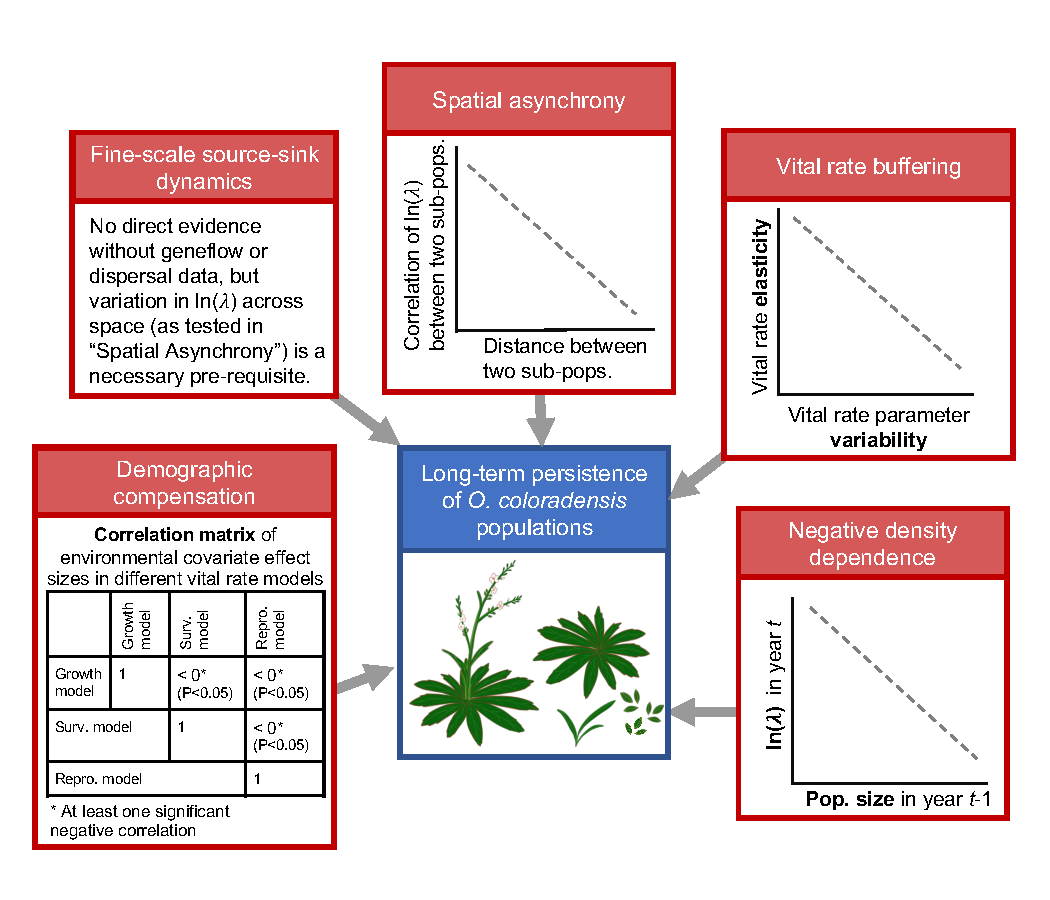
\includegraphics[width=1\textwidth]{COBP_conceptualDiagram.pdf}
  \caption{The evidence that would be required to show support for each of the five mechanisms that can contribute to the long-term viability of small populations of rare species.}
  \label{fig:conceptualFigure}
\end{figure} 

Here, we identify which mechanisms are contributing to the persistence or even population growth of a rare, endemic plant species, \textit{Oenothera coloradensis} (Onagraceae). We use integral projection models (IPMs) \cite{Easterling2000} that include a discrete seedbank population state. IPMs are flexible models of population dynamics that are constructed using regression models that describe vital rate change across a continuous state variable such as size. IPMs have multiple advantages including better performance with small datasets than traditional matrix models \cite{Ramula2009IntegralHerbs}, and simple incorporation of covariates of interest directly into vital rate models. Our first objective was to determine if including information about the seedbank significantly altered population models for \textit{O. coloradensis}. Seedbanks can serve as important reservoirs of genetic diversity and buffer populations against collapse \cite{Vitalis2004WhenPerenniality, Jongejans2006WhatRange}, and can be especially critical for monocarpic perennials that only flower once in their lifetime \cite{Rees2006}. For these reasons, we expected that a soil seedbank is important for \textit{O. coloradensis}. Seedbanks are often not included in population models because their parameters can be very difficult to estimate, but previous work shows that including them can significantly alter model outcomes \cite{Paniw2017, Nguyen2019ConsequencesModels}. We predicted that including a discrete seedbank state in IPMs would increase the projected $\lambda$ for \textit{O. coloradensis} populations. 

Our second objective was to identify whether any of the five persistence mechanisms was acting to maintain \textit{O. coloradensis} populations. This species occurs in habitats that naturally experience frequent, highly localized disturbance, which means that some subpopulations of \textit{O. coloradensis} might be negatively affected by flood, for example, while other nearby populations are simultaneously thriving due to lack of disturbance. Additionally, previous matrix population models constructed for this species in the 1990s found substantial variation in $\lambda$ across space and time \cite{Floyd1998}. The population-wide pattern of asynchronous habitat disturbance also could make source-sink dynamics important. We also have evidence of large fluctuations in the number of plants within subpopulations \cite{Heidel202133-YearWyoming}, which suggest that population growth rate decreases at high population size and increases at low population size. Therefore, we predicted that density dependence, small-scale source-sink dynamics and asynchronous responses between subpopulations would be important mechanisms of persistence for \textit{O. coloradensis}.  

\section{Methods}

\subsection{Species Description}  
\textit{Oenothera coloradensis} (Onagraceae) \cite{Wagner2013-ii} is an herbaceous, monocarpic perennial plant species that primarily occurs in frequently disturbed, mesic or wet meadows or riparian floodplains
\cite{Fertig2000-ow}. Non-reproductive individuals consist of a rosette of basal leaves with a fleshy taproot. Flowering typically occurs after several years of age around four years of age, when individuals produce a 10-30 cm long floral stalk. Individuals almost always die after reproducing—93\% of the time in populations we observed. \textit{O. coloradensis} populations typically occur within the floodplain of ephemeral or perennial streams, but also exist in wet meadows, and spring-fed wetlands \cite{Fertig2000-ow}. Relatively frequent disturbance such as flooding that reduces growth of both woody and herbaceous species and removes litter is important for this species, especially for successful seedling recruitment \cite{Fertig2000-ow, Burgess2003}. 

All historical and known extant \textit{O. coloradensis} populations lie within a 7,000-hectare area that includes southeast Wyoming, northern Colorado, and a small part of southwest Nebraska (Fig. \ref{fig:plotMap}). The only known population on Federal land occurs on the F. E. Warren Airforce Base near Cheyenne, WY (FEWAFB). The Soapstone Prairie Natural Area, a public property owned by the city of Fort Collins, CO, has the largest documented number of \textit{O. coloradensis} individuals, but this population has not been routinely monitored \cite{Heidel202133-YearWyoming}. Decline in a majority of the known populations between the mid-1980s and 2000 lead the U.S. Fish and Wildlife Service (USFWS) to designate \textit{O. coloradensis} as a “threatened” species protected under the Endangered Species Act (Endangered and Threatened Wildlife and Plants, 2000). Although this species appears to be naturally rare, mangers were concerned that, without protection, \textit{O. coloradensis} had the potential for extinction because of habitat loss due to ranching, natural resource extraction, and shrub encroachment resulting from altered disturbance regimes. However, based on additional monitoring following the initial listing decision, the USFWS determined that \textit{O. coloradensis} populations exhibit considerable natural variation in size, and that while monitored populations have both increased and decreased since the initial listing decision, the species as a whole does not appear to be on a trajectory toward extinction. As a result, \textit{O. coloradensis} was de-listed in 2019 (Endangered and Threatened Wildlife and Plants, 2019).
\nocite{USFWS2019}
\nocite{USFWS2000}


Previous work established that \textit{O. coloradensis} population growth rate is particularly impacted by recruitment of seedlings \cite{Floyd1998}. Seedbanks are also likely important for the viability of this species, since years of high seedling density are not necessarily preceded by years of high rates of flowering and seed production \cite{Munk2002RosetteSpecies, Heidel202133-YearWyoming}. The \textit{O. coloradensis} seedbank has not been studied directly, but a greenhouse seed viability and germination study showed that an average of 58\% of seeds produced by a parent plant are viable, and that a viable seed has a 20\% probability of germinating after two months of cold stratification \cite{Burgess2005CapsuleColoradensis}. These seed viability and germination rates did not change meaningfully over five years. 

More information about \textit{O. coloradensis} can be found in the Supplementary Material: "Species Information."

\subsection{Demographic Data Collection}
 We conducted a three-year demographic study of \textit{O. coloradensis} across six spatially distinct subpopulations, three in the F.E. Warren Airforce Base (FEWAFB) population and three at the Soapstone Prairie Natural Area population (Table \ref{plotLocationTable}; Fig. \ref{fig:plotMap}). In early summer 2018, we established three 2\textsf{x}2 m$^2$ quadrats in each of these subpopulations, resulting in 18 plots (Table \ref{plotLocationTable}) (Unnamed creek, Crow creek, and Diamond creek at FEWAFB and Meadow, Pasture HQ3 and Pasture HQ5 at Soapstone). Plants larger than 3 cm are typically "non-seedling" plants at least one year in age. In each study plot, we tagged and mapped each unique "non-seedling" individual and recorded longest leaf length, reproductive status, and seed production for each. Individuals smaller than 3 cm in leaf length are typically seedlings that germinated that year, occur at high density, and are less likely to survive than non-seedling plants. Due to these factors, we tallied seedlings in each plot, but did not map or tag them. In subsequent 2019 and 2020 censuses, we mapped and tagged new "non-seedling" individuals, and re-measured all surviving individuals from previous years. Sample size in a given year at a subpopulation ranged from 48 to 1527 individuals (Table \ref{plotLocationTable}). All mapping, tagging, and leaf measurements took place between late May and early July, coinciding with the peak of vegetative growth for this species. 

It was not possible to measure seed production exactly because \textit{O. coloradensis} seeds are contained in indehiscent capsules. Additionally, buds on the same individual flower and set seed with a time lag of up to several weeks, such that mature seed capsules often exist at the tip of a stem while un-opened buds lower down on that same stem have not yet flowered. This lag makes it difficult to count the total number of capsules produced by an individual. However, seed capsules leave a noticeable scar on the stem, so we used the number of seed capsule scars on reproductive stems as an estimate of capsule production. Counting scars is extremely time-intensive since a single plant can produce several hundred capsules, so we used Poisson generalized linear regression to estimate the relationship between the length of stem bearing capsule scars and the number of capsules produced by that stem. Poisson regression models fit to stem measurements and capsule counts from 106 individuals in 2018 indicates that the number of capsules produced by an indivdiual (C) can be predicted by $e^{(1.843 + 0.119\text{\textsf{x}}\text{S}))}$, where S is the stem length in cm (pseudo R-squared = 0.42, \textit{P} = $<$ 0.01, Resdiual deviance = 186.98, df = 104) (Fig. \ref{fig:seedRegression}). We used this relationship to estimate capsule production for each reproductive individual. Previous work indicated that each capsule contained an average of 4 seeds, so we multiplied the estimated number of capsules produced by an adult plant by 4 to estimate seed production \cite{Burgess2005CapsuleColoradensis}. 

\subsection{Environmental Measurements}
To determine the effect of temporal variation in climate on \textit{O. coloradensis} populations, we used modeled, site-level temperature, and precipitation data from PRISM \cite{PRISMClimateGroupOregonStateUniversity2021PRISMUniversity}, which we refer to as "environmental covariates". We calculated the mean temperature of both the growing season and preceding winter season for each year of demographic vital rate data collection at FEWAFB and Soapstone Prairie. We also calculated total precipitation for each hydrological year, the period from October of the previous year to September of the current year. We used this metric in place of growing season precipitation because the shortgrass steppe ecosystem in which \textit{O. coloradensis} occurs receives a majority of it's annual precipitation in the form of snow, and melting snow from the previous winter likely contributes to springtime seedling recruitment. Average temperature of the previous winter is also likely important for seedling recruitment, because seed germination is triggered by cold stratification \cite{Burgess2005CapsuleColoradensis}. Growing season temperature and precipitation are likely important for growth, survival, and reproductive output of non-seedling plants. 

\subsection{Objective 1: Quantifying the Importance of the Seedbank Stage}

\textit{Population Models}: We used data from the demographic study detailed above in combination with results from greenhouse and field seedbank studies to parameterize integral projection models (IPMs) for \textit{O. coloradensis}, which we then used to address each of the objectives outlined in the Introduction. We first created a density-independent IPM using data from both Soapstone and FEWAFB that had a single continuous, size-based population state, and did not include a seedbank state (Table \ref{IPMsTable}: IPM “A”). Then, we created a suite of IPMs that included both a discrete seedbank state, and a continuous, size-based stage for above-ground individuals (Table \ref{IPMsTable}: IPMs “A” – “NN”) \cite{Ellner2006IntegralDemography, Rees2006, Paniw2017}.  Each of these IPMs used a different subset of data, and included different covariates in vital rate models. First, the data used to fit vital rate models came either from a single subpopulation, a population (FEWAFB or Soapstone prairie), or from all locations, and included data for both transitions, or only one transition (2018-2019 or 2019-2020). Second, while all vital rate models included size in the current year (size$_t$)  (or in some cases when the model fitting process indicated, (size$_t$)$^2$) as a predictor of vital rates, these models could also include predictor terms for any combination of the following: population size in the previous year (to account for density dependence), environmental variation (water year precipitation, mean annual growing season temperature, and mean annual winter temperature), and a random intercept of subpopulation to approximate effects of demographic stochasticity.  

%\begin{table}
\small
\begin{spacing}{1.2}
\centering
%\resizebox{\textwidth}{!}{ 
\begin{longtable}{|p{0.028\textwidth}|p{0.02\textwidth} p{0.02\textwidth}|p{0.02\textwidth}| p{0.018\textwidth} p{0.018\textwidth} | p{0.018\textwidth} p{0.018\textwidth} p{0.018\textwidth} p{0.018\textwidth} p{0.018\textwidth} p{0.018\textwidth} 
|p{0.02\textwidth}|p{0.02\textwidth} p{0.02\textwidth}|p{0.04\textwidth}|p{0.04\textwidth}|p{2.55cm}|}   
\caption{A description of the data used to create each IPM, as well as the covariates included in the vital rate models used in that IPM. ln($\lambda$) estimates and 95\% bootstrap confidence intervals of ln($\lambda$) are also shown for each IPM.\label{IPMsTable}} \\
%\hline \\[-1.6ex] 
\toprule
\rotatebox{90}{IPM} & 
\multicolumn{11}{c}{Data Included} & 
\multicolumn{3}{|c}{Transition} & 
\multicolumn{2}{|c|}{Covariates} & 
\small ln($\lambda$) \hspace{2em} \footnotesize (95\% CI) 
\\ \cline{2-18}
& & & & \multicolumn{2}{|p{0.05\textwidth}|}{Each pop.} & \multicolumn{6}{c|}{Each subpop.} & & & & & &  \\\cline{5-12}
& \rotatebox{90}{Continuous state only} & \rotatebox{90}{Continuous + seedbank state} & \rotatebox{90}{All subpopulations} & \rotatebox{90}{Soapstone} & \rotatebox{90}{FEWAFB} & \rotatebox{90}{Unnamed Creek} & \rotatebox{90}{Diamond Creek} & \rotatebox{90}{Crow Creek} & \rotatebox{90}{Meadow} & \rotatebox{90}{HQ3} & \rotatebox{90}{HQ5} & \rotatebox{90}{All Transitions} & \rotatebox{90}{2018-2019} & \rotatebox{90}{2019-2020} & \rotatebox{90}{Density dependence} & \rotatebox{90}{Environmental covariates} &  \\
\hline
\rowcolor[gray]{.95} A&\textsf{x}&&\textsf{x}&&&&&&&&&\textsf{x}&&&&&0.27 \hspace{2em} \footnotesize (0.269, 0.271)  \\
B &&\textsf{x}&\textsf{x}&&&&&&&&&\textsf{x}&&&&&0.65 \hspace{2em} \footnotesize (0.648, 0.650)   \\
\rowcolor[gray]{.95}C&&\textsf{x}&&&&\textsf{x}&&&&&&\textsf{x}&&&&&0.48 \hspace{2em} \footnotesize  (0.477, 0.489) \\
D &&\textsf{x}&&&&&\textsf{x}&&&&&\textsf{x}&&&&& 1.13 \hspace{2em} \footnotesize  (1.124, 1.142)  \\
\rowcolor[gray]{.95} E &&\textsf{x}&&&&&&\textsf{x}&&&&\textsf{x}&&&&&0.74 \hspace{2em} \footnotesize  (0.725, 0.746) \\
F &&\textsf{x}&&&&&&&\textsf{x}&&&\textsf{x}&&&&&0.54 \hspace{2em} \footnotesize  (0.520, 0.551)  \\
\rowcolor[gray]{.95} G &&\textsf{x}&&&&&&&&\textsf{x}&&\textsf{x}&&&&&0.395 \hspace{2em} \footnotesize (0.378, 0.401)  \\
H &&\textsf{x}&&&&&&&&&\textsf{x}&\textsf{x}&&&&&0.53 \hspace{2em} \footnotesize (0.526, 0.540)  \\
\rowcolor[gray]{.95} I &&\textsf{x}&&&&\textsf{x}&&&&&&\textsf{x}&&&\textsf{x}&&0.59 \hspace{2em} \footnotesize (0.576, 0.637)  \\
J &&\textsf{x}&&&&&\textsf{x}&&&&&\textsf{x}&&&\textsf{x}&&0.63 \hspace{2em} \footnotesize (0.611, 0.723)  \\
\rowcolor[gray]{.95} K &&\textsf{x}&&&&&&\textsf{x}&&&&\textsf{x}&&&\textsf{x}&& $-0.10$ \hspace{2em} \footnotesize ($-0.135$, 0.063)  \\
L &&\textsf{x}&&&&&&&\textsf{x}&&&\textsf{x}&&&\textsf{x}&&$-0.20$ \hspace{2em} \footnotesize ($-0.229$, $-0.167$)  \\
\rowcolor[gray]{.95} M &&\textsf{x}&&&&&&&&\textsf{x}&&\textsf{x}&&&\textsf{x}&&1.31 \hspace{2em} \footnotesize (1.294, 1.354)  \\
N &&\textsf{x}&&&&&&&&&\textsf{x}&\textsf{x}&&&\textsf{x}&&2.31 \hspace{2em} \footnotesize (2.297, 2.33)  \\
%\rowcolor[gray]{.95} O &&\textsf{x}&&\textsf{x}&&&&&&&&\textsf{x}&&&\textsf{x}&\textsf{x}&\textsf{x}& n/a& 0.04 \\
%P \footnotesize hot/ dry &&\textsf{x}&&\textsf{x}&&&&&&&&\textsf{x}&&&\textsf{x}&\textsf{x}&\textsf{x}& n/a& 0.02\\
%\rowcolor[gray]{.95} Q &&\textsf{x}&&&\textsf{x}&&&&&&&\textsf{x}&&&\textsf{x}&\textsf{x}&\textsf{x}& n/a& 0.07 \\ 
%R \footnotesize hot/ dry &&\textsf{x}&&&\textsf{x}&&&&&&&\textsf{x}&&&\textsf{x}&\textsf{x}&\textsf{x}& n/a& 0.07 \\
\rowcolor[gray]{.95} S &&\textsf{x}&&&&\textsf{x}&&&&&&\textsf{x}&&&\textsf{x}&\textsf{x}&0.58 \\
T &&\textsf{x}&&&&&\textsf{x}&&&&&\textsf{x}&&&\textsf{x}&\textsf{x}&0.51 \\
\rowcolor[gray]{.95} U &&\textsf{x}&&&&&&\textsf{x}&&&&\textsf{x}&&&\textsf{x}&\textsf{x}&0.90 \\
V &&\textsf{x}&&&&&&&\textsf{x}&&&\textsf{x}&&&\textsf{x}&\textsf{x}&$-0.27$ \\
\rowcolor[gray]{.95} W &&\textsf{x}&&&&&&&&\textsf{x}&&\textsf{x}&&&\textsf{x}&\textsf{x}&$-0.18$ \\
X &&\textsf{x}&&&&&&&&&\textsf{x}&\textsf{x}&&&\textsf{x}&\textsf{x}&0.76 \\
\rowcolor[gray]{.95} AA &&\textsf{x}&&\textsf{x}&&&&&&&&\textsf{x}&&&&&0.50 \hspace{2em} \footnotesize (0.497, 0.501)  \\
BB &&\textsf{x}&&&\textsf{x}&&&&&&&\textsf{x}&&&&&0.73 \hspace{2em}  \footnotesize (0.729, 0.733)  \\
\rowcolor[gray]{.95} CC &&\textsf{x}&&&&\textsf{x}&&&&&&&\textsf{x}&&&&0.38 \hspace{2em} \footnotesize (0.370, 0.388)  \\
DD &&\textsf{x}&&&&&\textsf{x}&&&&&&\textsf{x}&&&&1.56 \hspace{2em} \footnotesize (1.545, 1.572)   \\
\rowcolor[gray]{.95} EE &&\textsf{x}&&&&&&\textsf{x}&&&&&\textsf{x}&&&&0.90 \hspace{2em} \footnotesize (0.864, 0.904)  \\
FF &&\textsf{x}&&&&&&&\textsf{x}&&&&\textsf{x}&&&&0.62 \hspace{2em} \footnotesize (0.592, 0.637)   \\
\rowcolor[gray]{.95} GG &&\textsf{x}&&&&&&&&\textsf{x}&&&\textsf{x}&&&&0.73 \hspace{2em} \footnotesize (0.727, 0.753)  \\
HH &&\textsf{x}&&&&&&&&&\textsf{x}&&\textsf{x}&&&&1.11 \hspace{2em} \footnotesize (1.108, 1.126)  \\
\rowcolor[gray]{.95} II &&\textsf{x}&&&&\textsf{x}&&&&&&&&\textsf{x}&&&0.50 \hspace{2em} \footnotesize (0.492, 0.513)  \\
JJ &&\textsf{x}&&&&&\textsf{x}&&&&&&&\textsf{x}&&&0.71 \hspace{2em} \footnotesize (0.692, 0.726)   \\
\rowcolor[gray]{.95} KK &&\textsf{x}&&&&&&\textsf{x}&&&&&&\textsf{x}&&&0.76 \hspace{2em} \footnotesize (0.739, 0.774)   \\
LL &&\textsf{x}&&&&&&&\textsf{x}&&&&&\textsf{x}&&&0.41 \hspace{2em} \footnotesize (0.378, 0.448)   \\
\rowcolor[gray]{.95} MM &&\textsf{x}&&&&&&&&\textsf{x}&&&&\textsf{x}&&&0.03   \hspace{2em} \footnotesize (0.013, 0.040)   \\
NN &&\textsf{x}&&&&&&&&&\textsf{x}&&&\textsf{x}&&&$-0.10$ \hspace{2em} \footnotesize ($-0.112$, $-0.097$)    \\
\hline
\multicolumn{18}{p{.96\textwidth}}{*Note: We did not calculate bootstrap 95\% confidence intervals for ln($\lambda$) of models “S” –“X”, since only vital rate parameters and not lambda values from these models were used in further analysis. }
\end{longtable}
\end{spacing}

\normalsize{}
The IPM with one state variable corresponding to continuous plant size (IPM “A”) used a kernel structure where the continuous, above-ground population state (($n(z’, t+1)$) at time $t+1$ was described by the following equation:  
\begin{equation}\label{eqn:oneStateIPM}
n(z', t+1) = \int_{L}^{U}(1-P_b(z))s(z)G(z',z)n(z,t)dz + pEstab\int_{L}^{U}P_b(z)b(z)c_o(z')n(z,t)dz
\end{equation}
All of the IPMs with two population states used the same kernel structure, where the continuous, above-ground population state ($n(z',t+1)$) and the seedbank state ($B(t+1)$) at time $t+1$ were described by the following equations: 
\begin{equation}\label{eqn:twoStateIPM_cont}
n(z', t+1) = \int_{L}^{U}(1-P_b(z))s(z)G(z',z)n(z,t)dz + goCont\int_{L}^{U}P_b(z)b(z)c_o(z')n(z,t)dz + outSB 
\end{equation}
\begin{equation}\label{eqn:twoStateIPM_disc}
     B(t+1) = goSB\int_{L}^{U}P_b(z)b(z)n(z,t)dz + B(t)staySB 
\end{equation}

In both sets of equations, $z$ is the distribution of plant longest leaf length in the current year (“$size_t$”), $z’$ is the distribution of plant size in the next year (“$size_{t+1}$”), and $U$ and $L$ are the upper and lower boundaries of plant size. $G(z’, z)$ is the vital rate function describing $size_{t+1}$ as a function of $size_t$. The vital rate functions $s(z)$, $Pb(z)$, and $b(z)$ describe the relationship between $size_t$ and survival probability of non-flowering plants, flowering probability, and seed production of flowering plants, respectively.  $c_o(z’)$ is the distribution of above-ground recruit $size_{t+1}$. $goCont$, $outSB$, $goSB$, and $staySB$ are discrete parameters that determine seedbank dynamics. $goCont$ is the probability of a seed produced in year $t$ germinating as a seedling in year $t+1$, $outSB$ is the probability of a seed from the seedbank in year $t$ germinating as a seedling in year $t+1$, $goSB$ is the probability of a seed produced in year $t$ going into the seedbank in year $t+1$, and $staySB$ is the probability of a seed from the seedbank in year $t$ persisting in the seedbank in year $t+1$ \cite{Paniw2017} (Table \ref{table:VitalRates}). $pEstab$ is the probability of a seed produced in year $t$ establishing as a seedling in year $t+1$.  

We used data from the three-year demographic monitoring study to parameterize the vital rates used in the IPMs (vital rates are shown in Fig. \ref{fig:lifecycle}). Vital rate functions for the continuous, size-based above-ground stage were parameterized using data from “non-seedling plants” as well as seedlings. Although seedlings (above-ground plants $<$ 3 cm in leaf length) were only tallied in each subplot of each quadrat and year instead of tagged and measured, we incorporated them into the dataset for continuous, above-ground plants by assigning them a random size drawn from a continuous, uniform probability distribution (seedling size $\sim U($0.1, 3)). Each new recruit to the $>$ 3 cm stage in year $t+1$ was randomly assigned to a seedling within the same subplot in year $t$. Seedlings in year $t$ that were assigned a recruit in year $t+1$ survived, while those without an assigned recruit died. Incorporating seedlings into the continuous dataset in this fashion allowed us to create IPMs using only one discrete stage.  

We used data from the demographic study to estimate continuous vital rate functions describing survival, growth, probability of flowering, seed production, and recruit size. For each of these vital rates, we fit subpopulation-level models as well as models using data across all sites. We additionally fit models with and without density dependence, with and without environmental covariates, and using data either from all years or from each unique annual transition. The basic model structure was the same for each vital rate (Table \ref{table:VitalRates}). All models included log-transformed leaf $size_t$ as a predictor. Log-transformed leaf $size_t$ squared was also included as a predictor if it decreased model AIC. Additional covariates indicating population size and environmental conditions were added to these basic models. 

We modeled survival probability ($s(z)$) as a function of log-transformed leaf $size_t$ using generalized linear models with binomial error distributions. Flowering individuals were excluded from the data used to fit survival models, since \textit{O. coloradensis} is a monocarpic perennial that nearly always dies after flowering. Probability of flowering ($Pb(z)$) was also modeled using generalized linear models with binomial error distributions, and was predicted by log-transformed leaf $size_t$ plus log-transformed leaf $size_t$ squared. We estimated seed production ($b(z)$) as a function of $size_t$ using negative binomial models because the count data was over-dispersed. We only used data from flowering plants in this analysis, and fit these models using the “glm.nb” function from the “MASS” R package \cite{Venables2002ModernS}. Plant $size_{t+1}$ ($G(z’,z)$) was described as a series of Normal distributions with mean = $\mu_s$ and standard deviation = $\sigma_s$. Mean plant $size_{t+1}$ ($\mu_s$) was modeled as a function of $size_t$ using linear models with Gaussian error. The standard deviation of plant $size_{t+1}$ ($\sigma_s$) was the residual standard error of these linear models, which we assumed to be constant. The distributions of recruit size in the next year ($c_o(z’)$) were described by Normal distributions with the mean $\mu_r$, and the standard deviation $\sigma_r$. $\mu_r$ and $\sigma_r$ were the mean and standard deviation of observed plant size in the next year. 

\begin{figure}[h]
    \centering
    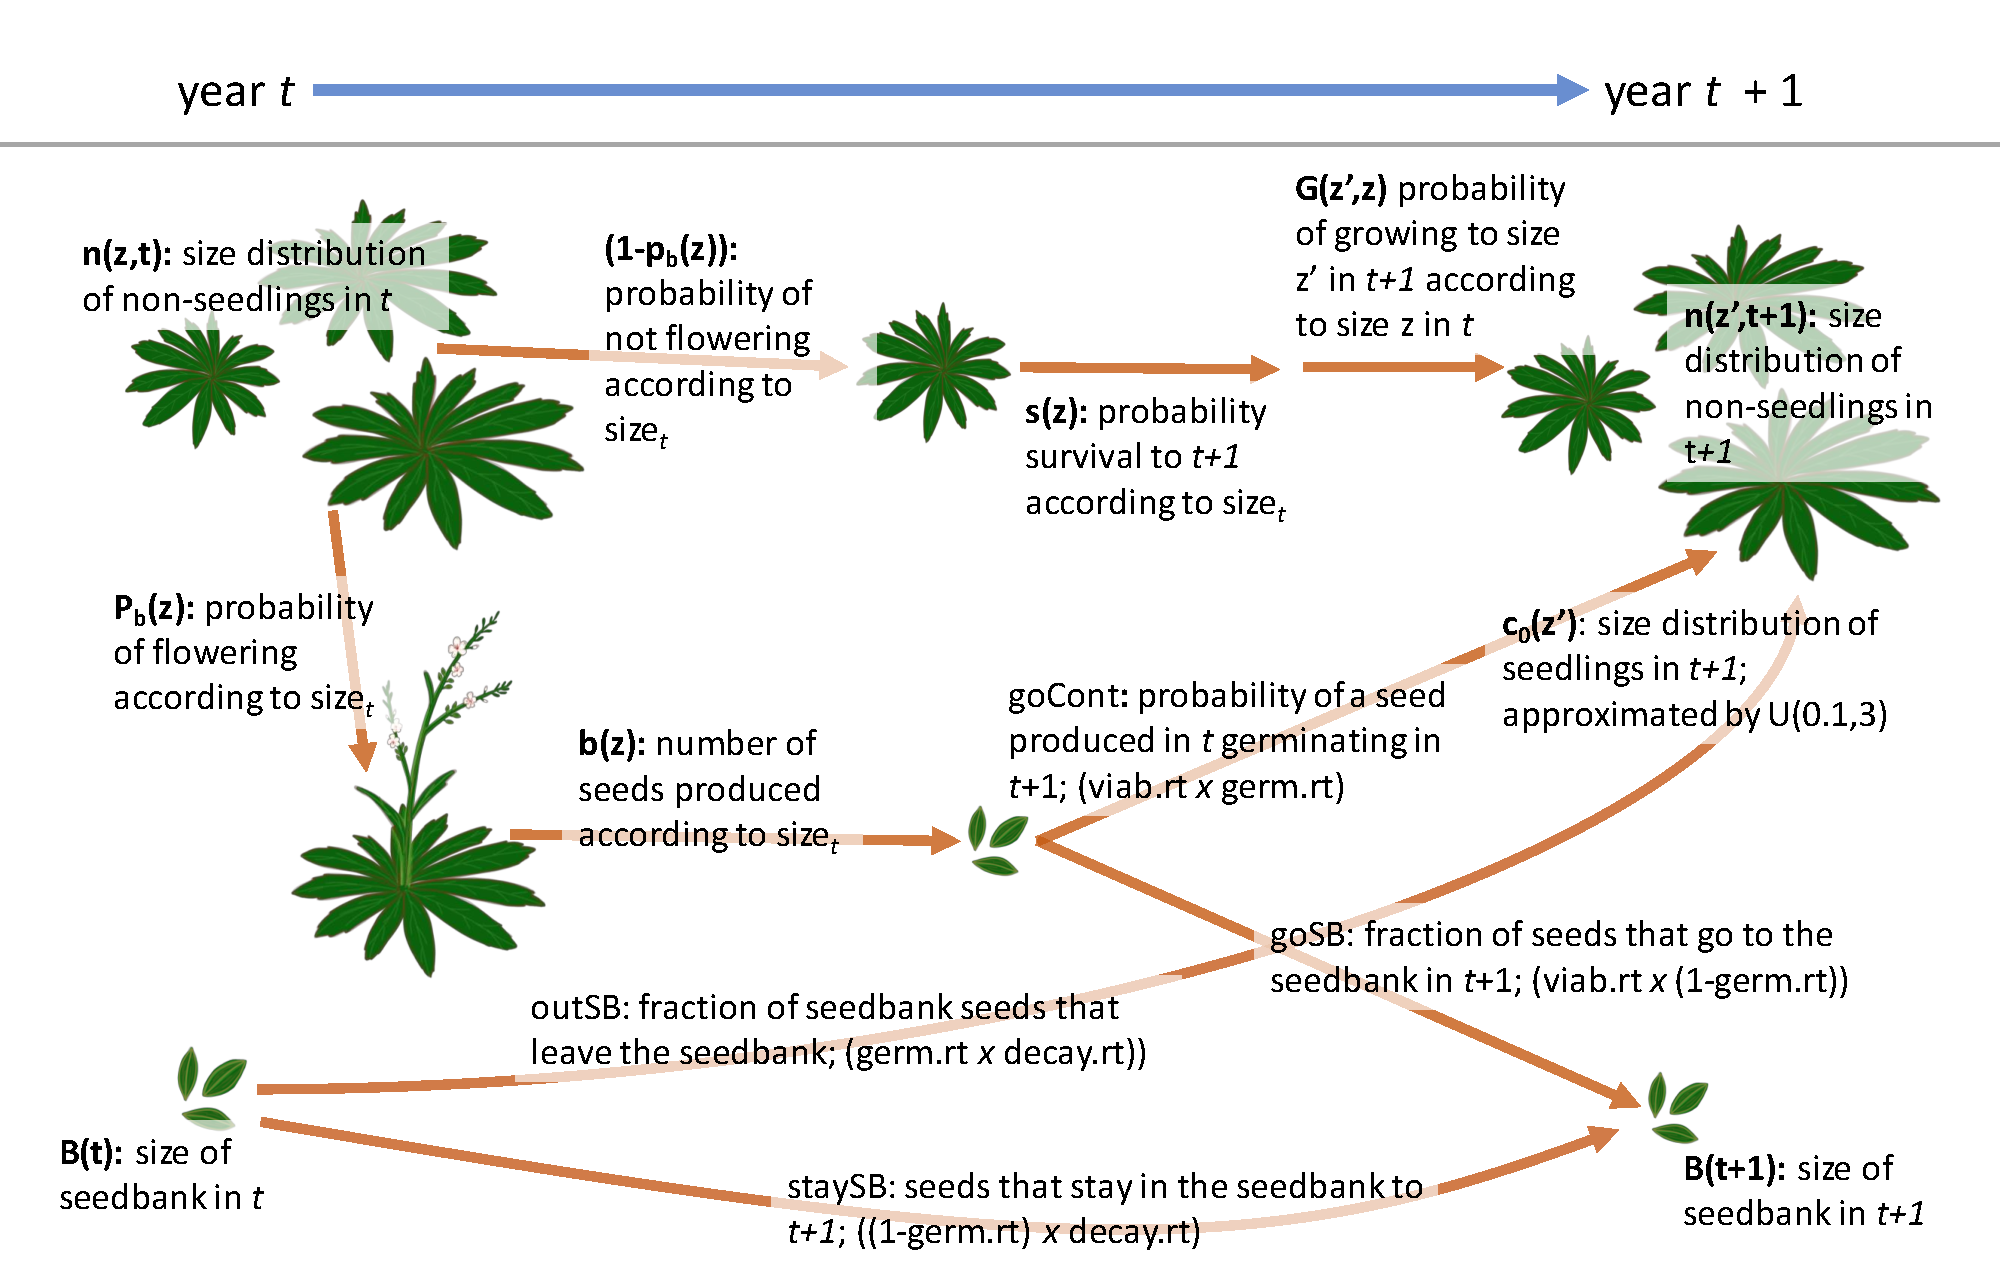
\includegraphics[width=1\textwidth]{COBP_lifecyclediagram_new.pdf}
    \caption{Diagram of the \textit{O. coloradensis} life-cycle, with transitions labeled with the notation used in IPM equations. Based on model structures and notation from: \cite{Paniw2017, Merow2014AdvancingGuide, Ellner2016Data-drivenPopulations}. "germ.rt" = germination rate, "viab.rt" = viability rate, "decay.rt" = decay rate.}
    \label{fig:lifecycle}
\end{figure}

\begin{table}[h]
\centering
\begin{spacing}{1.3}
\caption{Description of vital rates used in \textit{O. coloradensis} IPMs\label{table:VitalRates}}
\begin{tabular}{L{0.16\textwidth}p{0.28\textwidth}p{0.5\textwidth}}
\toprule
Vital Rate & Description & Model \\
\hline
\rowcolor[gray]{.95} \textit{pEstab} & \small\textit{P}(seed produced in \textit{t} establishes as a seedling in \textit{t+1}) & $pEstab$ = $\frac{Num.\;new\;recruits\;in\;year_{t+1}}{Num.\;seeds\;produced\;in\;year_t}$\\

\textit{goCont} & \small \textit{P}(seed produced in \textit{t} germinates in \textit{t+1}) & $goCont$ = viab. rate \textsf{x} germ. rate\\
\rowcolor[gray]{.95} 
\textit{outSB} & \small\textit{P}(seedbank seed in \textit{t} germinates in \textit{t+1}) & $outSB$ = germ. rate \textsf{x} ($1 - $death rate)\\

\textit{goSB} & \small\textit{P}(seed produced in \textit{t} goes into the seedbank in \textit{t+1}) & $goSB$ = viab. rate \textsf{x} ($1 - $germ. rate)\\
\rowcolor[gray]{.95} 
\textit{staySB} & \small\textit{P}(seedbank seed in \textit{t} stays in the seedbank in \textit{t+1}) & $staySB$ = ($1-$ germ. rate) \textsf{x} ($1 - $death rate)\\
\textit{Survival (s(z))} & \small\textit{P}(survival from \textit{t} to \textit{t+1}) & logit(survival) $\sim \beta_0 + \beta_1 (ln(size_t)) + \epsilon$\\ 
\rowcolor[gray]{.95} 
 \textit{Flowering (Pb(z))} & \small\textit{P}(flowering in \textit{t}) & logit(flowering) $\sim \beta_0 + \beta_1 (ln(size_t)) + \beta_2 (ln(size_t)^2) + \epsilon$\\ 
 \textit{Seed prod. (b(z))} & \small Seed production in \textit{t} & exp(seed number) $\sim \beta_0 + \beta_1 (ln(size_t)) +  \epsilon$\\ 
\rowcolor[gray]{.95} 
\textit{Growth (G(z',z))} & \small Distribution of plant size in year \textit{t} & $G(z',z) = N(\mu_s, \sigma_s); \newline \mu_s \sim \beta_0 + \beta_1 (ln(size_t)) + \epsilon; \newline \sigma_s \sim RSE(\beta_0 + \beta_1 (ln(size_t)) + \epsilon)$\\ 
 \textit{Recruit size ($c_o$(z'))} & \small Distribution of new recruit size in year \textit{t} & $c_o(z') = N(\mu_r, \sigma_r); \newline \mu_r = $mean(size of recruits in $t); \newline \sigma_r = $stnd. dev. (size of recruits in $t)$\\
\hline
\multicolumn{3}{l}{* RSE = residual standard error} 
\end{tabular}
\end{spacing}
\end{table}

We estimated discrete vital rates for seeds using data from both greenhouse and field-based germination and seed viability studies. Previously-published data from a greenhouse experiment using \textit{O. coloradensis} seed capsules collected from the FEWAFB populations determined that viable seeds had an average germination rate of 20.3\% after cold-stratification, and did not identify a consistent decline in germination rate over five years (Burgess et al. 2005). This study also found that a seed capsule contained an average of 1.7 seeds, and that 58.5\% of seeds produced were viable. We conducted an additional seed study to determine if overwintering in natural conditions lead to a lower germination rate than was identified in the previous greenhouse study. We buried 60 field-collected seed capsules in mesh bags at 6 locations near our demographic study plots at FEWAFB, and then recovered the seed bags after one winter. An average of 10\% of seed capsules were not recoverable, likely because they were non-viable and withered away or were eaten. We planted the recovered capsules in standard greenhouse conditions, and found a mean germination rate of 6.8\%. This germination rate was much lower than that identified by Burgess et al., however our seed study had a much smaller sample size, reducing the reliability of our result. However, it is still likely that true germination rates are much lower than those identified in greenhouse conditions, so we reduced the germination rate identified by Burgess et al. by 20\%. The following parameters we used to estimate the discrete seed vital rate parameters: viable seed germination rate (germ. rate) = 0.16, viability rate of seeds produced by a parent plant (viab. rate) = 0.58, rate of natural seed death in the seedbank (death rate) = 0.10. We did not have the data required to determine how these rates changed across subpopulations or in response to abiotic variation, so we used the same seed vital rates for all IPM models (Table \ref{table:VitalRates}).  

We used these vital rate functions and discrete parameters described above to construct discretized IPM kernels. All kernels were numerically implemented using the “midpoint rule” method \cite{Easterling2000} with 500 bins, an upper size limit corresponding to 120\% of the maximum observed plant size and a lower size limit corresponding to 80\% of the minimum simulated seedling size of 0.1 cm. We then used eigen analysis of these kernels to estimate the asymptotic population growth rate ($\lambda$), damping ratio, stable size distribution, and reproductive value \cite{Caswell2001MatrixInterpretation, Ellner2016Data-drivenPopulations}. We used 1000 iterations of bootstrap re-sampling to estimate 95\% bootstrap confidence intervals (95\% CIs) for each continuous vital rate parameter included in each IPM, as well as each estimate of $\lambda$ \cite{Merow2014AdvancingGuide, Fieberg2020Resampling-basedBiologists}. We were unable to estimate CIs for discrete seedbank parameters because they were drawn from a previous publication. We used perturbation analysis to determine the sensitivity and elasticity of $\lambda$ to changes in germination rate, viability rate, seed survival rate, and each parameter in each continuous vital rate model \cite{Morris2002QuantitativeAnalysis}. We used the IPM with all data and no density dependence or environmental covariates (IPM “B”) for this analysis. All vital rate models and IPMs, as well as the information derived from them, were used to evaluate the importance of negative density dependence, demographic compensation, vital rate buffering, asynchronous responses, and source-sink dynamics for persistence of \textit{O. coloradensis} populations.  

\subsection{Objective 2: Evaluating Persistence Mechanisms}

\textit{Negative Density Dependence:} In order to determine the importance of density dependence in \textit{O. coloradensis} subpopulations, we compared subpopulation-level, all-transition IPMs and vital rate functions that did and did not include population size in the current year as a covariate in vital rate models (density-independent IPMs: “C”-“H” in Table \ref{IPMsTable}; density-dependent IPMs: “I”-“N”). We used AIC to identify significant differences between vital rate models with and without density dependence terms. We also used results from subpopulation-level IPMs (Table \ref{IPMsTable}: IPMs "CC"-"NN") for each transition to identify relationships between subpopulation size in year \textit{t}  and ln($\lambda$) (as in Fig. \ref{fig:conceptualFigure}), as well as subpopulation size in year \textit{t} and the ratio of population size in year \textit{t+1 }and subpopulation size in year \textit{t}. In addition to population size information and ln($\lambda$) values from our IPMs, we also used population sizes and ln($\lambda$) values from a previously-published demographic study of \textit{O. coloradensis} at the three FEWAFB subpopulations that we also monitored \cite{Floyd1998}.  A negative relationship between population size in year \textit{t} and either ln($\lambda$) or the ratio of population size in year \textit{t + 1} to population size in year \textit{t} would provide evidence for negative density dependence. Additionally, significant differences between models with and without population size predictor terms would constitute evidence for density dependence.  

\textit{Demographic Compensation:} To test for demographic compensation, we calculated the correlation between environmental covariate coefficients in different vital rate models. A negative correlation between coefficients of the same covariate in different vital rate models indicated demographic compensation was taking place \cite{Villellas2015DemographicImplications, Dibner2019}. For example, if soil moisture had a positive effect on growth but a negative effect on survival, this would be evidence for demographic compensation. For this correlation analysis we used vital rate models that were fit using data from each subpopulation and both transitions, and that included covariates for density dependence and all environmental covariates (vital rate models from IPMs “S”-“X” in Table \ref{IPMsTable}). We tested the significance of negative correlations between environmental covariate coefficients using a randomization procedure similar to that used by Villellas et al. (2015), where we randomly assigned an environmental covariate coefficient drawn from the observed distribution of values for that coefficient to each vital rate function, calculated a correlation matrix between those coefficients in each vital rate function, and counted the number of negative correlations in that matrix. This procedure was repeated 10,000 times to generate a null distribution of the expected number of negative correlations between environmental coefficients that would occur randomly. We compared the observed number of negative correlations between each environmental covariate coefficient to these expected distributions of random correlations to determine statistical significance. We could not test for demographic compensation in discrete seedbank vital rate parameters because we did not know how they varied according to environmental conditions.  A significant negative correlation between environmental covariate coefficients in different vital rate models would provide evidence for demographic compensation (Fig. \ref{fig:conceptualFigure}).  


\textit{Vital Rate Buffering:} We tested for the presence of vital rate buffering in \textit{O. coloradensis} populations by comparing the variability of demographic rates to their importance. We used an approach that scales both the standard deviation (variability metric) and sensitivity (importance metric) of vital rates, allowing for a fair comparison of variability and importance across vital rates with fundamentally different relationships between their mean and variance \cite{McDonald2017DivergentEnvironments}. Vital rates that are probabilities (i.e. survival, flowering, growth, discrete seedbank transition probabilities, and seedling size) are constrained between zero and one and thus typically have small variance as the mean approaches these limits, while other vital rates are only constrained by zero and thus typically have variances that increase as the mean increases (i.e. seed productivity) \cite{Gaillard2003-ch}. To enable a fair comparison between these different categories of vital rates, we calculated the importance and variability of probability and non-probability vital rates in different ways. The importance of probability vital rates was defined as the logit variance stabilized sensitivity, and the variability was defined by the standard deviation of the logit transformed vital rate values \cite{McDonald2017DivergentEnvironments, William_A_Link_Paul_F_Doherty_Fr2002-cb}. The importance of non-probability vital rates was defined as the log-scaled sensitivity (or elasticity), and the variability was defined by the standard deviation of the log-transformed vital rate values \cite{McDonald2017DivergentEnvironments, Morris2002QuantitativeAnalysis}.

We used an IPM that was fit across all subpopulations using data from both transitions (Table \ref{IPMsTable}: IPM “B”) to calculate elasticity or logit VSS values for each discrete vital rate and continuous vital rate function. 
We calculated the scaled standard deviation for each continuous vital rate function using the vital rates that were fit uniquely for each subpopulation and each transition (Table \ref{IPMsTable}: IPMs “CC”-“NN”). Because we did not have site-level information about discrete seedbank vital rates, we simulated both the maximum and minimum possible standard deviations for each discrete vital rate. We then proceeded with two comparisons of vital rate variability and importance, once using the maximum possible discrete vital rate standard deviation, and another using the minimum. In order to determine the correlation between a single importance/variability value pair for discrete vital rates and a string of value pairs for continuous vital rate functions, we calculated mean importance and variability values for each continuous vital rate function. A significant negative correlation between the mean or absolute scaled importance (logit VSS or elasiticity) and mean or absolute variability (standard deviation of logit or log-transformed vital rates) across all vital rates would constitute support for the presence of vital rate buffering in this species
(Fig. \ref{fig:conceptualFigure}).  

\textit{Asynchronous Responses and Source-Sink Dynamics:} To determine whether \textit{O. coloradensis} subpopulations showed asynchronous responses to environmental variation, we made a correlation matrix to determine how change in ln($\lambda$) across each transition was correlated across each subpopulation, using values of ln($\lambda$) derived from IPMs for each subpopulation (Table \ref{IPMsTable}: IPMs “C”-“H”). We used the “mantel()” function from the “vegan” R package to perform a Mantel test, which determined if the Spearman correlation of ln($\lambda$) across subpopulations was significantly related to the Euclidian distance between each subpopulation \cite{Oksanen2020Vegan:Package}. A negative relationship between the distance between subpopulations and degree of correlation of ln($\lambda$) would constitute evidence for spatial asynchrony between subpopulations (Fig. \ref{fig:conceptualFigure}).   

Because we did not have information about gene flow between subpopulations of \textit{O. coloradensis} via pollination or seed dispersal, it was not possible to directly measure whether fine-scale source-sink dynamics were acting in these populations. However, because variation in population growth rate across space is a pre-requisite for source-sink dynamics, the previously described tests for spatial asynchrony in subpopulations can also provide evidence for the existence of source-sink dynamics. Again, this would be a negative relationship of distance between subpopulations and correlation of subpopulation ln($\lambda$) (Fig. \ref{fig:conceptualFigure}).  

%\subsection{Objective 3: Population Viability Analysis}

% To determine the likelihood that each population (Soapstone prairie and FEWAFB) would persist, we used the “ipmr” R package to project each population forward 50 years, incorporating the effects of density dependence and demographic and environmental stochasticity (using IPMs “O”-“R”) \cite{Levin2021Ipmr:R}. Each projection was repeated 1000 times, and stochastic ln($\lambda$) (or ln($\lambda_s$)) was calculated with a burn-in of 15 iterations. We did one set of projections using climate values that were randomly drawn from the distribution of observed climate values at each population site. A second set of projections drew climate values from distributions that were 10\% warmer and 10\% drier than the observed climate, to evaluate how \textit{O. coloradensis} populations may fare under hotter and drier conditions that are predicted to occur in this region under climate change \cite{Vicente-Serrano2020AWarming}.  
 
\section{Results}

\subsection{Vital Rate Models} 

In vital rate models parameterized for each population using data from both transitions, we found that larger non-reproductive plants are more likely to survive to year \textit{t+1} than smaller plants (Fig. \ref{fig:vitalRates}A). Plants below ~7.5 cm in year \textit{t} are likely to become larger in year \textit{t+1}, while plants larger than ~7.5 cm are likely to become smaller in the next year (Fig. \ref{fig:vitalRates} B). Flowering probability is best approximated as a quadratic polynomial: flowering probability rises when ln(size$_t$) approaches 2.5 (12 cm), but plants with the largest leaves exhibit low flowering probability (Fig. \ref{fig:vitalRates} C). The number of seeds that a reproductive plant produces increases sharply with ln(size$_t$) (Fig. \ref{fig:vitalRates} D). The inclusion of additional covariates did not alter the overall shape or sign of the relationships between ln(size$_t$) and vital rates, so models shown in Figure \ref{fig:vitalRates} did not include any additional covariates beyond ln(size$_t$).  

\begin{figure}[h]
  \centering
  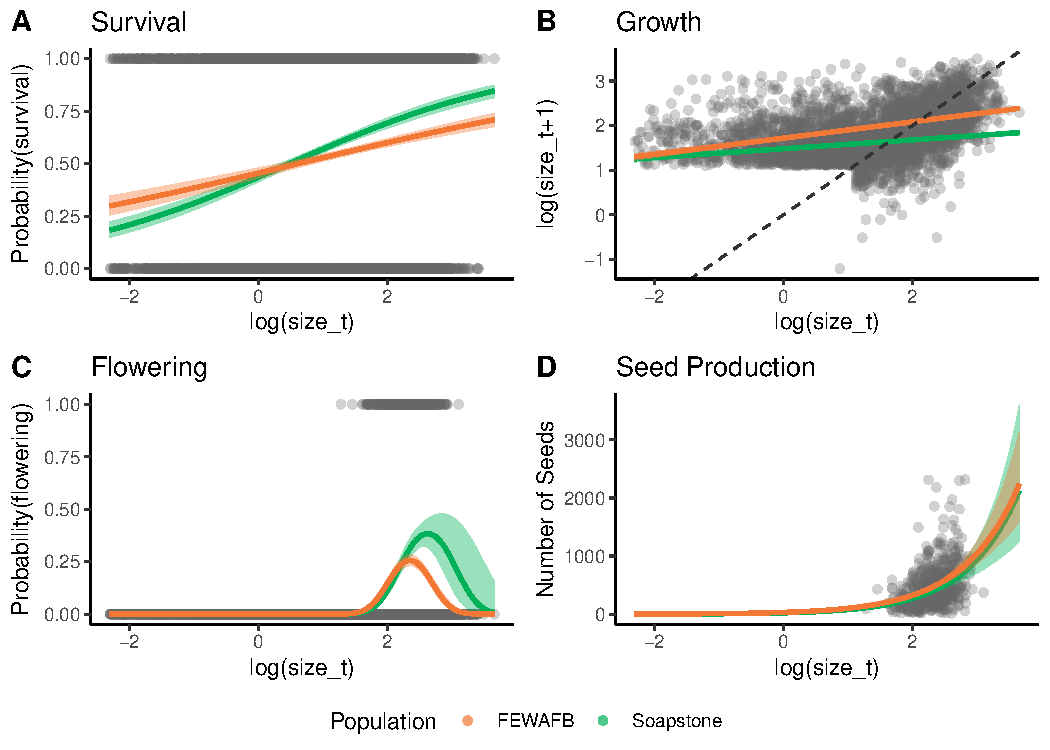
\includegraphics[width=\textwidth]{figures/vitalRateModelFit.pdf}
  \caption{The effect of current year size (ln(size$_t$)) on vital rates in monitored \textit{O. coloradensis} populations. Data for from all sites and all transitions is shown. Lines indicate vital rate functions for each population, and include only ln(size$_t$) as a predictor, with the exception of flowering models, which include a (ln(size$_t$))$^2$ term. Bands around each line show 95\% confidence intervals. The dashed line in panel \textbf{B} shows a 1:1 line. The sharp cut-off in ln(size$_{t+1}$) in panel \textbf{B} is due to the fact that two-year-old plants could not be seedlings, which were classified as any plant less than 3 cm in size.}
  \label{fig:vitalRates}
\end{figure} 

\subsection{Objective 1: Quantifying the Importance of the Seedbank Stage}

\textit{Integral Projection Models:} We found that including a discrete seedbank stage in IPMs for \textit{O. coloradensis} significantly increased the asymptotic population growth rate. The continuous state-only IPM (Table \ref{IPMsTable}: IPM “A”) predicted an asymptotic ln($\lambda$) of 0.27 for all populations (95\% CI: 0.269 - 0.271), while the continuous + discrete state IPM (Table \ref{IPMsTable}: IPM “B”) predicted an asymptotic ln($\lambda$) of 0.65 (populations (95\% CI: 0.648 - 0.650). All subsequent IPM results refer to models that included a discrete seedbank state. 

The simplest two-state IPMs that excluded density dependence and environmental variation indicated that both the Soapstone prairie and FEWAFB populations had positive population growth rates (Table \ref{IPMsTable}: Soapstone prairie- IPM “AA”, ln($\lambda$) = 0.50;  FEWAFB – IPM “BB”, ln($\lambda$) =  0.73). The Diamond Creek subpopulation at FEWAFB had the highest population growth rate from 2018 to 2020 (Table \ref{IPMsTable}: IPM “D”, ln($\lambda$) = 0.1.13), while the HQ3 subpopulation at Soapstone prairie had the lowest growth rate (Table \ref{IPMsTable}: IPM “G”, ln($\lambda$) = 0.395). We parameterized multiple other sets of IPMs that used different combinations of covariates in their vital rate models, and almost all identified a positive population growth rate (Table \ref{IPMsTable}).   

A density-independent, discretized IPM kernel (made using IPM “B” in Table \ref{IPMsTable}) shows transition probabilities within and between the discrete and continuous stages of the O. coloradensis lifecycle when all populations and transitions are considered together (Fig. \ref{fig:IPMKernel} A). Relative to the rest of the kernel, there is a very high probability that seeds stay in the seedbank, as well as a large contribution of seeds from medium-sized adult plants to the seedbank in the next year. The rates at which seeds are produced by adult plants and stay in the seedbank have the most impact on population growth rate (Fig. \ref{fig:IPMKernel} C).

\begin{figure}[h]
  \centering
  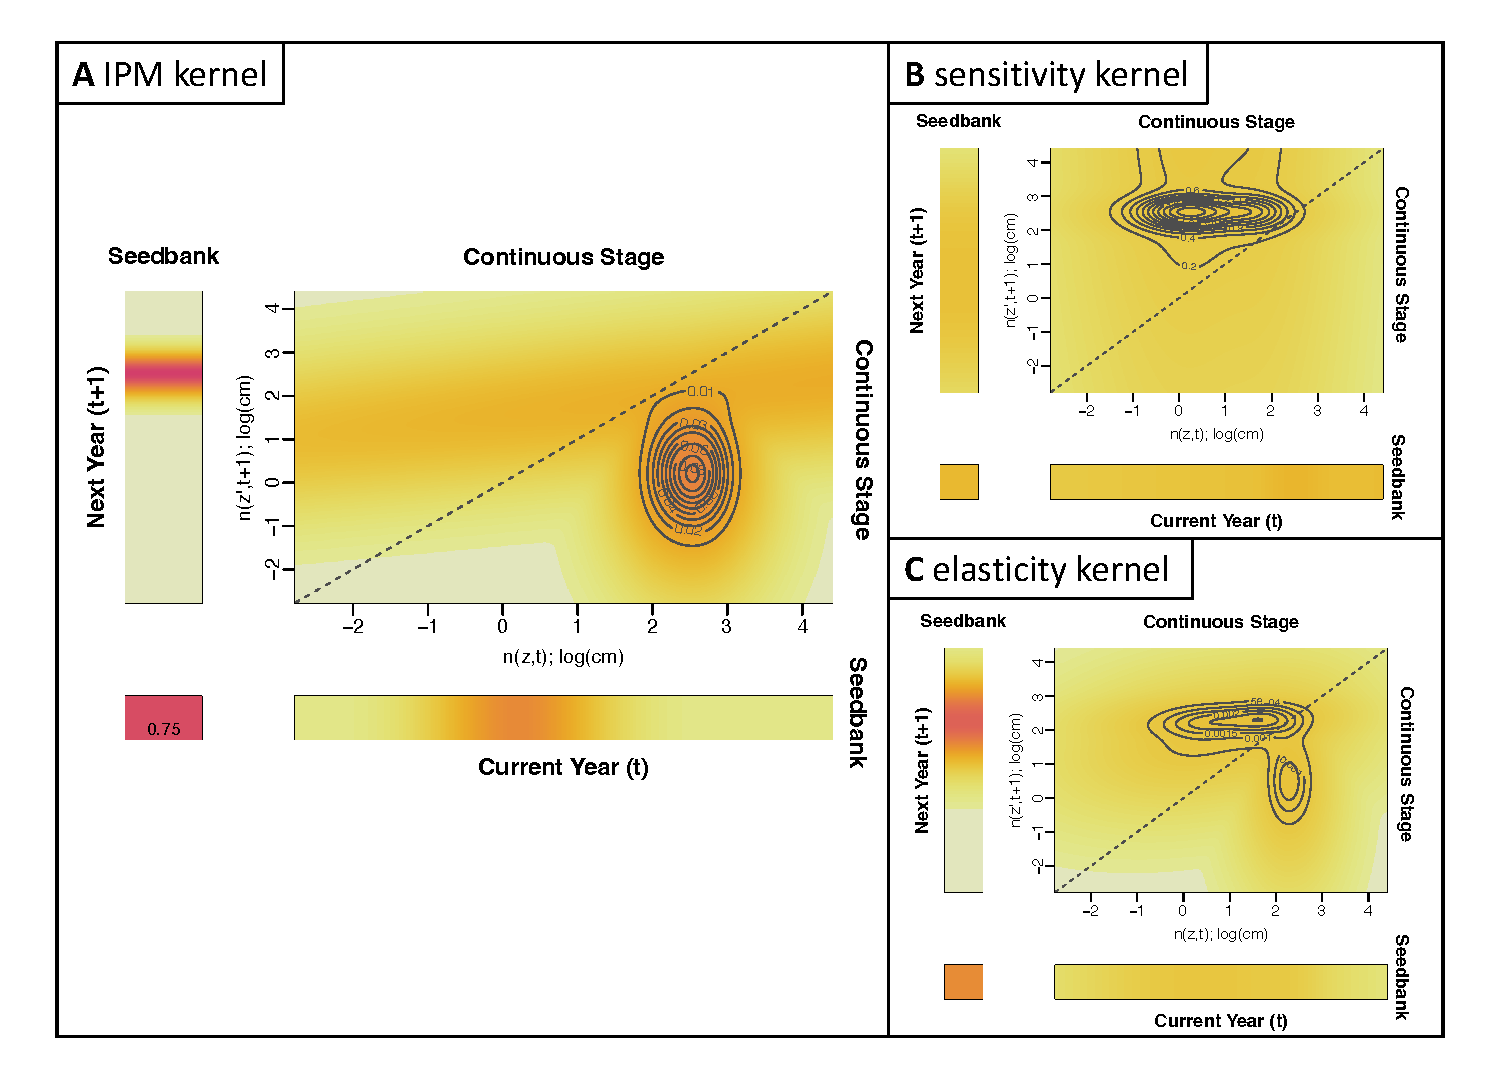
\includegraphics[width=\textwidth]{figures/KernelMultipanelFigure.pdf}
  \caption{Visualizations of the \textit{O. coloradensis} IPM kernels. \textbf{A} The IPM kernel for \textit{O. coloradensis}. This kernel shows a density-independent IPM constructed using all data from all transitions (IPM "B"). \textbf{B} Sensitivity of the IPM kernel. \textbf{C} Elasticity of the IPM kernel. In all panels, color indicates probability, with darker colors corresponding to higher probability, and lighter colors corresponding to lower probability. The dashed line shows a 1:1 line. }
  \label{fig:IPMKernel}
\end{figure} 

\subsection{Objective 2: Evaluating Persistence Mechanisms}

\textit{Negative Density Dependence:} There is moderate evidence that negative density-dependence is acting to maintain populations of \textit{O. coloradensis}. AIC comparison of continuous vital rate models indicate that density-dependent models are better predictors of the majority of vital rates than density-independent models in most subpopulations (Table \ref{Table:DDModResults}).  Models that included population size in the previous year as a covariate were better predictors of growth in five of six subpopulations. Density dependent models were better predictors of survival and seed production than density independent models in four out of six subpopulations, and density dependent models of flowering were better in one subpopulation. Recruit size distribution was not affected by density dependence—AIC model comparison did not indicate substantial differences, either negative or positive, between recruit size models with and without density dependence terms in any subpopulation. The vital rate models for the Meadow population at Soapstone Prairie were least affected by density dependence. Although density dependence is important for \textit{O. coloradensis} in many situations, it appears only to be acting to decrease lambda at high density (as in the highly dense Diamond Creek or HQ5 subpopulations), but not clearly increasing lambda at low density (as in the sparsely populated Meadow subpopulation). We also found that population growth rate is generally higher when population size is smaller, but only when comparing the relationship between ln($\lambda$) and population size within a subpopulation (Fig. \ref{fig:DDFig} A and C). There is also a negative relationship within each subpopulation between population size in year \textit{t} and the ratio of subpopulation size in \textit{t+1} to subpopulation size in \textit{t} (Fig. \ref{fig:DDFig} B and D). However, when looking across all subpopulations, there is not a clear relationship between subpopulation size in \textit{t} and either ln($\lambda$) or the ratio of subpopulation size in \textit{t+1}.  

\begin{table}[h]
\centering
\begin{spacing}{1.2}
\caption{Comparison of vital rate models that do and do not include density dependence. The “DI” and “DD” rows contain AIC values for each vital rate model in each subpopulation for models that are density-independent (DI) and density-dependent (DD). The difference between the AIC of DI and DD models is shown in the $\Delta$AIC column. Bold text indicates that the $|\Delta|$AIC value is $>$ 3, which means that including a term for density dependence substantially changed that vital rate model. A positive $|\Delta|$AIC indicates that including density dependence improved the model, while a negative value indicates that including density dependence made model fit worse.\label{Table:DDModResults}}
\begin{tabular}{l l p{.08\textwidth} p{.1\textwidth} p{.1\textwidth}ccc}
\toprule
\multicolumn{2}{c}{Vital Rate Model} & \multicolumn{6}{c}{Subpopulation} 
\\ \cline{3-8}
& & Crow Creek & Diamond Creek & Unnamed Creek & HQ5 & HQ3 & Meadow \\ 
\hline
\rowcolor[gray]{.95} Survival & DI &     776.58 &  1012.68 & 2684.34 & 3242.63 & 716.66 & 166.13 \\
\rowcolor[gray]{.95} & DD &              757.84 &  905.39  & 26848.74 & 2922.91 & 637.84 & 166.83 \\ 
\rowcolor[gray]{.95} & $\Delta$AIC &     \textbf{18.74} &   \textbf{107.28} &  -0.41 &   \textbf{320.33} &  \textbf{78.82} &   -0.70 \\ 
Growth & DI &                            510.34 &  953.29 &  1098.95 & 1570.93 & 300.18 & 116.54 \\
& DD &                                   506.61 &  931.15 &  1068.14 & 1112.78 & 269.73 & 113.88 \\
& $\Delta$AIC &                          \textbf{3.73} &    \textbf{22.15} &   \textbf{30.811} &  \textbf{458.15} &  \textbf{30.45} &  2.66 \\
\rowcolor[gray]{.95} Flowering & DI &    371.68 &  523.30 &  1087.93 & 538.52 &  191.46 & 104.24 \\
\rowcolor[gray]{.95} & DD &              373.31 &  523.74  & 1087.48 & 483.99 &  193.22 & 106.96 \\
\rowcolor[gray]{.95} & $\Delta$AIC &     -1.63 &   -0.44 &   0.45 &    \textbf{54.52} &   -1.76 &  -1.72 \\
Seed production & DI &                   842.00 &  1580.85 & 2815.89 & 1423.02 & 598.75 & 280.09 \\
& DD &                                   835.59 &  1566.83 & 2817.19 & 1419.32 & 594.63 & 281.45 \\
 & $\Delta$AIC &                         \textbf{6.41} &    \textbf{14.02} &   -1.29 &   \textbf{3.71} &    \textbf{4.12} &   -1.35 \\ 
\rowcolor[gray]{.95} Recruit size & DI & 921.31 &  1028.23 & 3378.43 & 4629.87 & 967.83 & 173.03 \\
\rowcolor[gray]{.95} & DD &              923.24 &  1026.63 & 3380.53 & 4631.84 & 969.06 & 175.02 \\ 
\rowcolor[gray]{.95} & $\Delta$AIC &     -1.93 &   1.61 &   -1.93 &   -1.97 &   -1.23 &  -1.99 \\
\hline
\end{tabular}
\end{spacing}
\end{table}

\begin{figure}[h]
  \centering
  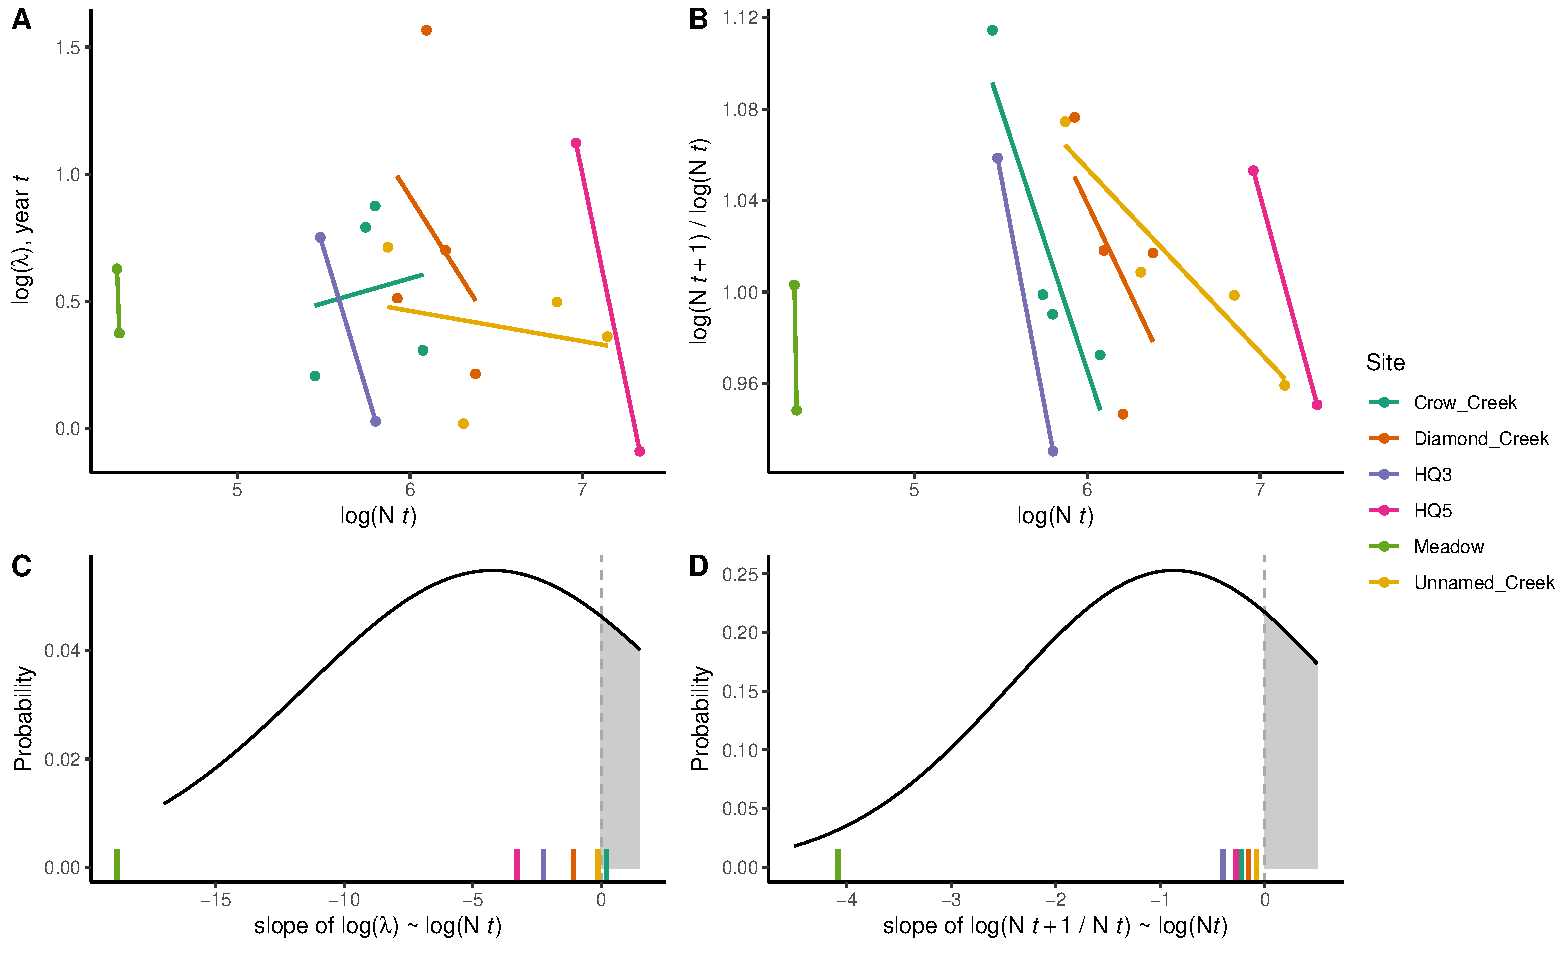
\includegraphics[width=.8\textwidth]{figures/densityDependenceFigure.pdf}
  \caption{\textbf{A} Within the same subpopulation, population growth rate (ln($\lambda$)) calculated from IPMs decreases as population size increases. \textbf{B} Population growth rate calculated by change in population size from year \textit{t} to year \textit{t+1} also decreases as population size increases in the same subpopulation. In \textbf{A} and \textbf{B}, each point represents values calculated from data from one transition in one subpopulation. Lines show linear regressions of the relationships between ln(N$_t$) and the respective response variable in each subpopulation. Rug plots in panels \textbf{C} and \textbf{D} show the slope of each regression line in panels \textbf{A} and \textbf{B}, respectively. The normal distributions in \textbf{C} and \textbf{D} were created using the means and standard deviations of these slopes. According to these distributions of observed slopes, there is a 28\% probability that the true relationship between ln($\lambda$) and ln(N$_t$) is positive, and a 29\% probability that the true relationship between ln(N$_t$) and ln(N$_{t+1}$/N$_t$) is positive. In all panels, “N” indicates the number of individuals in a subpopulation. }
  \label{fig:DDFig}
\end{figure} 

\textit{Demographic Compensation:} Our analyses did not identify signatures of demographic compensation in \textit{O. coloradensis} populations. While there were negative correlations between the effect of mean growing season temperature on vital rates for five combinations of vital rates, none of these correlations were significant (Table \ref{Table:DemoComp}). The only significant correlation was positive. Ten thousand correlations of randomly assigned coefficients found that the number of negative correlations in a matrix can be described by a normal distribution with a mean of 4.97 and a standard deviation of 1.60. Using this distribution as a null model, there was a 50.7\% probability of observing five negative correlations. Although there is no significant evidence for demographic compensation, it is notable that the effect of mean growing season temperature on distribution of recruit size was negatively correlated with the effect of growing season temperature on all other vital rates. We were only able to compare coefficients across vital rate models for mean growing season temperature, because including precipitation and mean winter temperature as covariates resulted in overfitting in some cases.  

\begin{table}[h]
\centering
\begin{spacing}{1.2}
\caption{Pearson correlations between mean growing season temperature coefficients in each continuous vital rate function. Below each correlation value is the \textit{P} value for that correlation. Bold text indicates a significant correlation. \label{Table:DemoComp}}
\begin{tabular}{p{.03\textwidth} c p{.1\textwidth} p{.1\textwidth} p{.1\textwidth} p{.1\textwidth} p{.1\textwidth}}
\toprule
& & \multicolumn{2}{c}{\textbf{Vital Rate}} \\ 
\cline{3-7}
& & \textit{Flowering} & \textit{Survival} & \textit{Growth} & \textit{Seed Prod.} & \textit{Recruit Size} \\ 
\hline
\multirow{5}{*}{\rotatebox{90}{\textbf{Vital Rate} }} & \cellcolor[gray]{.95}\textit{Flowering} & \cellcolor[gray]{.95}1.00 \:\:\: (0) & \cellcolor[gray]{.95}0.474 (0.342) & \cellcolor[gray]{.95}0.136 (0.797) & \cellcolor[gray]{.95}-0.073 (0.890) & \cellcolor[gray]{.95}-0.786 \: (0.064) \\
& \multicolumn{2}{r}{\textit{Survival}} &  1.00 \: \: (0) & 0.886 \textbf{(0.019)} & 0.675 (0.141) & -0.3570 \:(0.237) \\
 &  \multicolumn{3}{r}{\textit{\cellcolor[gray]{.95} Growth}} & \cellcolor[gray]{.95} 1.00 \: \: (0) & \cellcolor[gray]{.95} 0.664 (0.150) & \cellcolor[gray]{.95} -0.270  \:  (0.606) \\
& \multicolumn{4}{r}{\textit{Seed Prod.}} & 1.00 \:\:\: (0) & -0.432 \: (0.393) \\
 & \multicolumn{5}{r}{\cellcolor[gray]{.95}\textit{Recruit Size}} & \cellcolor[gray]{.95} 1.00 \:\:\:\:\: (0)\\
\hline
\end{tabular}
\end{spacing}
\end{table}

\textit{Vital Rate Buffering:} We did not identify strong evidence of vital rate buffering in the \textit{O. coloradensis} populations we observed. 
Vital rate importance (either logistic VSS or elasticity) and variability (corrected SD) were not significantly negatively correlated, regardless of the simulated standard deviation for discrete vital rates we used(Fig. \ref{fig:VRBuffering}; correlation with minimum discrete vital rate SD (\textbf{A}): \textit{r} = 0.43 , \textit{P} = 0.25; correlation with maximum discrete vital rate SD (\textbf{B}): \textit{r} = -0.07 , \textit{P} = 0.85). As a vital rate became more important for determining population growth rate, it did not become significantly less variable, showing no evidence that vital rate buffering is taking place (Fig. \ref{fig:conceptualFigure}).  

\begin{figure}[h]
  \centering
  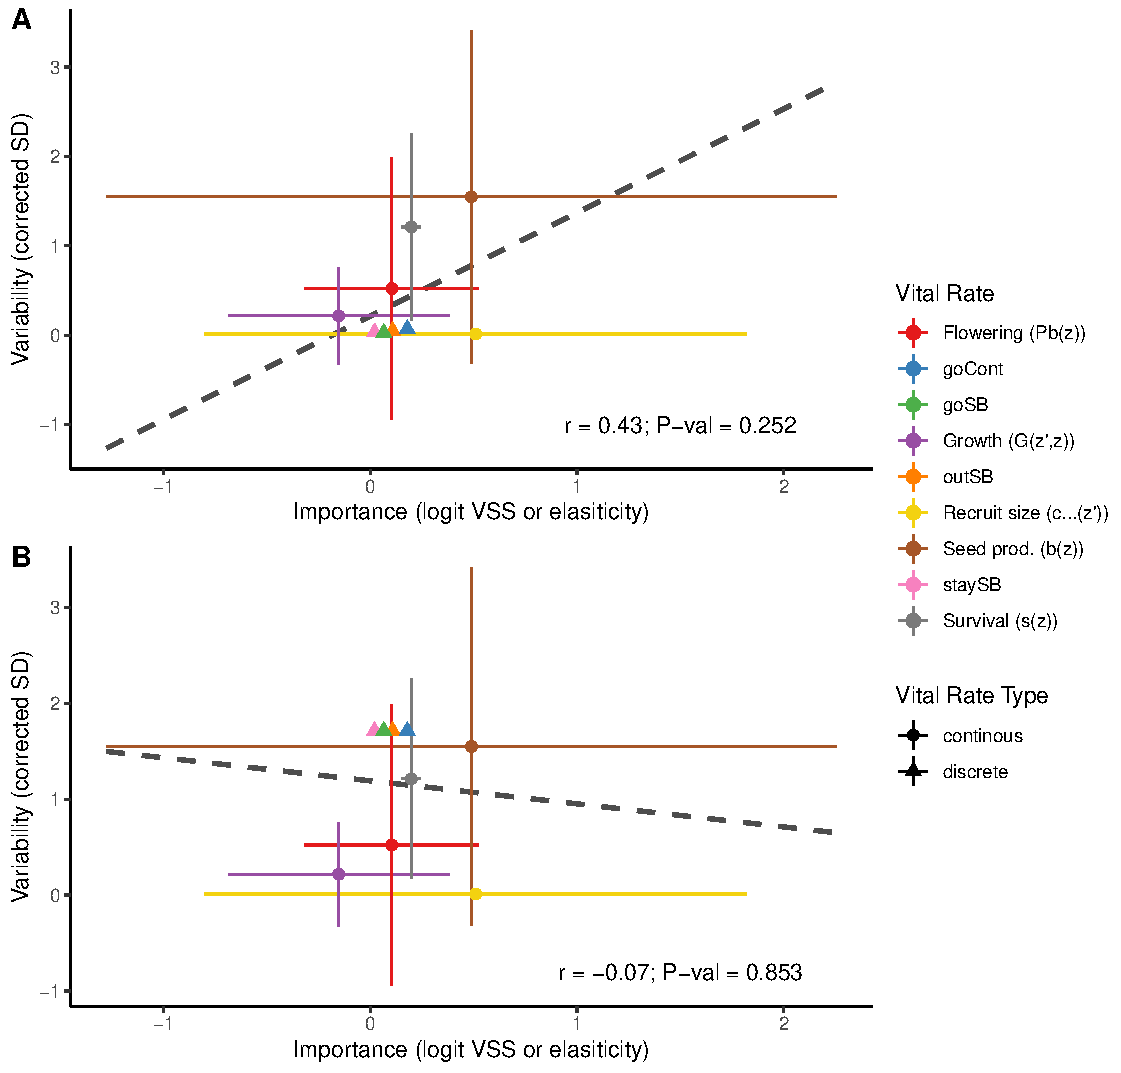
\includegraphics[width=.7\textwidth]{figures/VRbufferingFigure.pdf}
  \caption{The relationship between the variability of each vital rate (measured by corrected standard deviation) and its importance (measured by logit VSS or elasticity) does not show support for vital rate buffering. In these figures, a triangle indicates importance and variability for a discrete vital rate parameter, while a circle indicates the mean of importance and variability across an entire continuous vital rate function. Error bars around continuous vital rate means span the the 5$^{th}$ to 95$^{th}$ percentiles of either importance or variability values calculated for an entire continuous vital rate function. Dashed lines show the correlation between (mean) variability and (mean) importance across all vital rates. Because we lacked data to calculate the actual standard deviation of discrete vital rates, we simulated both the minimum and maximum possible standard deviation for each of these rates. (\textbf{A}) With the minimum possible discrete vital rate variability, there is a positive but insignificant correlation between vital rate variability and importance ( \textit{r} = 0.43 , \textit{P} = 0.25). (\textbf{B}) Using the maximum possible discrete vital rate variability, there is a negative but insignificant correlation between vital rate variability and importance (\textit{r} = -0.07 , \textit{P} = 0.85).}
  \label{fig:VRBuffering}
\end{figure} 

\textit{Asynchronous Responses and Source-Sink Dynamics:} We did not identify a signature of asynchronous responses to environmental variation in \textit{O. coloradensis} populations. There was not a significant relationship between the Spearman correlation of ln($\lambda$) between subpopulations and their spatial proximity (Mantel statistic = 0.396, \textit{P} = 0.06). We also performed Mantel tests using ln($\lambda$) correlation and distance matrices calculated uniquely for each population. There was not a significant relationship between subpopulation growth rate and spatial proximity at either Soapstone prairie (Mantel statistic = -0.659, \textit{P} = 0.83) or FEWAFB (Mantel statistic = 0.798, \textit{P} = 0.33). While these tests did not identify significant relationships, we did find a positive relationship between correlation of ln($\lambda$) and distance between subpopulations at Soapstone prairie, and a negative relationship between subpopulations at FEWAFB. Collectively, these results fail to provide support for both asynchronous responses and fine-scale source-sink dynamics in these O. coloradensis populations. 

%\subsection{Objective 3: Population Viability Analysis}

 %Simulations that incorporate demographic and environmental stochasticity and density dependence indicate that, if the demographic patterns observed during our monitoring study persist, both the Soapstone prairie and FEWAFB populations of \textit{O. coloradensis} will hover around their current population size for the next decade (Fig. \ref{fig:Simulation} A; Table \ref{Table:SimCoeffs}). Over a span of 50 years, however, the simulations suggest that the Soapstone population will grow considerably to reach an equilibrium size that is an order of magnitude larger than it is currently, and the FEWAFB population will grow exponentially and then decline steadily through the end of the simulation period. By the end of the simulations, the population growth rate of the Soapstone population stabilizes slightly above zero, while the growth rate of the FEWAFB population stabilizes slightly below zero (Fig. \ref{fig:Simulation} B). Even though the FEWAFB population is in decline at the end of the simulation period, the mean stochastic ln($\lambda$) (or ln($\lambda_s$), which is the mean of the ln($\lambda$) values of the 15th through 50th simulated transitions, is positive. This is driven by the very high ln($\lambda$) values in the first 30 years of the simulations (Fig. \ref{fig:Simulation} C). The mean ln($\lambda_s$) for the Soapstone population is lower than the FEWAFB ln($\lambda_s$), but is still positive. 

%The climate scenario used for the simulation did not substantially affect the outcome for the FEWAFB populations. Mean population size, mean ln($\lambda$) and ln($\lambda_s$) of the FEWAFB population are very similar both in simulations using a scenario based on current observed climate and a scenario with higher mean temperature and lower precipitation. However, climate scenario did affect the outcome of simulations of the Soapstone prairie population. In the hotter and drier scenario, population size grew faster initially, but stabilized at a smaller size than in the current climate scenario (Fig. \ref{fig:Simulation} B). Mean ln($\lambda_s$) was also lower in the hotter and drier climate scenario (Fig. \ref{fig:Simulation} C).  

%\begin{figure}[h]
%  \centering
%  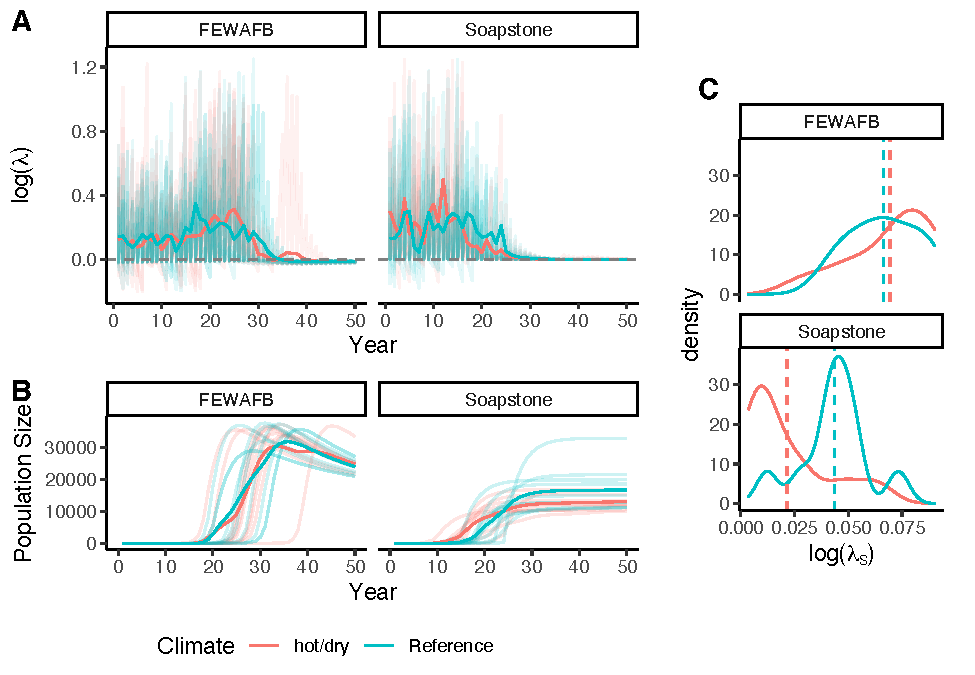
\includegraphics[width=\textwidth]{figures/SimulationFigure.pdf}
%  \caption{Simulated growth rates and sizes of each population under two climate scenarios. \textbf{A} Simulated ln($\lambda$) of the Soapstone prairie population stabilizes just above zero in both climate scenarios after $~$30 years. Simulated ln($\lambda$) of the FEWAFB population stabilizes just below zero after $~$40 years. Solid, dark-colored lines show the mean ln($\lambda$) at each simulated transition, while faint lines show ln($\lambda$) values for each iteration of the simulation. Horizontal dashed lines indicate ln($\lambda_s$) = 0. \textbf{B} Simulated size of the Soapstone prairie population grows until reaching an equilibrium size, which is smaller in the hotter and drier climate scenario. Simulated size of the FEWAFB population grows initially, but is still in decline at the end of the simulation period. \textbf{C} Climate scenario does not have a pronounced effect on the distribution of observed stochastic $\lambda$ (ln($\lambda_s$)) values in simulations of the FEWAFB population. In simulations of the Soapstone prairie population, mean ln($\lambda_s$) is lower under the hotter and drier climate scenario. Vertical dashed lines indicate mean ln($\lambda_s$) under each climate scenario.}
%  \label{fig:Simulation}
%\end{figure}

%\begin{table}[h]
%\centering
%\begin{spacing}{1.2}
%\caption{Coefficients from vital rate models that were used to create projection IPMs. "Density" column refers to plot-level plant density; "Temp." column refers to mean growing season temperature; "Precip." column refers to total water-year precipitation; "Subpop. rand.-int." column refers to subpopulation random intercept \label{Table:SimCoeffs}}
%\begin{tabular}{p{.018\textwidth} p{.11\textwidth}  | p{.08\textwidth} p{.08\textwidth} p{.08\textwidth} p{.1\textwidth} p{.1\textwidth} p{.08\textwidth} | p{.11\textwidth}}
%\toprule
%& & \multicolumn{6}{p{.5\textwidth}}{Coefficient \:\:\:\:\:\:\:\:\:\:\:\:\:\:\:\:\:\:\:\:\:\:\:\:\:\:\:\:\:\:\:\:\:\:\:\:\:\:\:\:\:\:\:\:\:\:\:\:\:\:\:\:\:\:\:\:\:\:\:\:\:\:\:\:\:\: \small (\textit{P}-value)} & \multicolumn{1}{|p{.11\textwidth}}{Variance \small(std. dev.)} \\ 
%\cline{3-9}
%& Response Variable & \small Intercept & \small ln(size$_t$) &  \small ln(size$_t$)$^2$ & \small Density & \small Temp. & \small Precip. & \small Subpop. rand.-int.\\
%\hline
% & \cellcolor[gray]{.95} \small P(survival) & \cellcolor[gray]{.95}\small -0.21 (0.48) & \cellcolor[gray]{.95}\small 0.73 ($<$0.01) \cellcolor[gray]{.95}\small & \cellcolor[gray]{.95}- & \cellcolor[gray]{.95}\small 0.002  \:\: ($<$0.01) & \cellcolor[gray]{.95}\small 0.82 \: \:\:\:\: ($<$0.01) & \cellcolor[gray]{.95}\small - & \cellcolor[gray]{.95}\small 0.24 \: (0.49) \\
%\multirow{5}{*}{\rotatebox{90}{Soapstone Prairie}}& \small ln(size$_{t+1}$) & \small 1.56 ($<$0.01) & \small 0.17    ($<$0.01) & \small - & \small -3.8x10$^{-5}$ (0.39) & \small 0.21  ($<$0.01) & \small - & \small 0.01 \: (0.10) \\
% & \cellcolor[gray]{.95} \small P(flower) & \cellcolor[gray]{.95} \small -30.77  ($<$0.01) & \cellcolor[gray]{.95} \small 23.13   ($<$0.01) & \cellcolor[gray]{.95} \small -4.34   ($<$0.01) & \cellcolor[gray]{.95} \small 0.0014 ($<$0.01) & \cellcolor[gray]{.95} \small 0.50  ($<$0.01) & \cellcolor[gray]{.95} \small -0.14  (0.47) & \cellcolor[gray]{.95} \small 0.24  \:(0.49) \\
%& \small Num. seeds & \small 3.89 ($<$0.01) & \small  0.39 (0.07) & \small - & \small 0.0006 ($<$0.01) & \small 0.38  ($<$0.01) & \small 0.83  ($<$0.01) & \small  - \\
%& \cellcolor[gray]{.95}\small Recruit Size & \cellcolor[gray]{.95}\small 0.23  ($<$0.01) & \cellcolor[gray]{.95}\small - & \cellcolor[gray]{.95}\small - & \cellcolor[gray]{.95}\small -7.6x10$^{-6}$ (0.90) & \cellcolor[gray]{.95}\small -4.5x10$^{-3}$ (0.80) & \cellcolor[gray]{.95}\small -0.002 (0.45) & \cellcolor[gray]{.95}\small - \\
%\hline
%& \small P(survival) & \small -1.07 (0.08) & \small 0.27  ($<$0.01) & \small - & \small 0.005  ($<$0.01) & \small 0.20  ($<$0.01) & \small - & \small 1.07 \: (1.03) \\
%\multirow{5}{*}{\rotatebox{90}{FEWAFB}} & \cellcolor[gray]{.95} \small ln(size$_{t+1}$)  & \cellcolor[gray]{.95} \small 1.62 ($<$0.01) & \cellcolor[gray]{.95} \small  0.19  ($<$0.01) & \cellcolor[gray]{.95} \small - & \cellcolor[gray]{.95} \small 5.08x10$^{-4}$  ($<$0.01) & \cellcolor[gray]{.95} \small -0.02 (0.14) & \cellcolor[gray]{.95} \small - & \cellcolor[gray]{.95} \small 0.09 \: (0.30) \\
%& \small P(flower) & \small -30.12  ($<$0.01) & \small 27.38  ($<$0.01) & \small -5.88  ($<$0.01) & \small 3.95x10$^{-4}$  (0.45) & \small 0.11 (0.09) & \small0.22 ($<$0.01) & \small0.07 \: (0.26) \\
% & \cellcolor[gray]{.95}\small Num. seeds & \cellcolor[gray]{.95}\small 3.13  ($<$0.01) & \cellcolor[gray]{.95}\small 0.90  ($<$0.01) & \cellcolor[gray]{.95}\small -  & \cellcolor[gray]{.95}\small -0.0001 (0.56) & \cellcolor[gray]{.95}\small 0.11 ($<$0.01) & \cellcolor[gray]{.95}\small 0.11 ($<$0.01) & \cellcolor[gray]{.95}\small - \\  
%& \small Recruit Size & \small 0.19  ($<$0.01) & \small - & \small - & \small -1.2x10$^{-5}$ (0.89) & \small 0.03    (0.10) & \small -0.006 (0.68)  & \small - \\
%\hline
%\end{tabular}
%\end{spacing}
%\end{table}

\section{Discussion}
\normalfont Our demographic analysis of the two largest known populations of the globally rare \textit{Oenothera coloradensis} evaluated the importance of seedbanks to population dynamics and identified the demographic mechanisms that allow this rare species to persist. First, we found that including information about cryptic life stages alters the outcomes of the population model \cite{Paniw2017, Nguyen2019ConsequencesModels}. \textit{O. coloradensis} populations show signs of negative density-dependence at the subpopulation scale (Fig. \ref{fig:DDFig}; Table \ref{Table:DDModResults}). However, these populations do not show substantial evidence of demographic compensation, vital rate buffering, spatial asynchrony, or fine-scale source-sink dynamics. This may indicate that while these mechanisms may be important for the persistence of many small populations of rare plants, they are not strictly necessary in all cases. 

Including a discrete seedbank state in an IPM increased the asymptotic population growth rate compared to an IPM with only a continuous, size-based state, although both growth rates were still positive (Table \ref{IPMsTable}: with seedbank: IPM “B”, ln($\lambda$) = 0.65; without seedbank: IPM “A”, ln($\lambda$) = 0.27). The importance of the including the seedbank in the model aligned with our expectations, and also align with the conventional notion that seedbanks can act as buffers against stochastic causes of population decline. The discrete rates for the probability of persisting and transitioning out of the seedbank have high elasticity in the IPMs in which they are included, but not the highest elasticity of any vital rate(Fig. \ref{fig:IPMKernel} C). The rate at which seeds produced by adult plants in year \textit{t} go into the seedbank in year \textit{t+1} is the vital rate function with highest elasticity. Previous matrix population models of \textit{O. coloradensis} without a seedbank state that were constructed in the 1990s identified the emergence rate of new seedlings as the vital rate most important for determining ln($\lambda$) \cite{Floyd1998}. Our finding that seedbank state transitions are important for this species aligns with this previous result, since rate of seedling emergence is the above-ground plant vital rate that is closest to the seedbank in this plant’s life cycle. An important caveat to our comparison of models with and without seedbank stages is the fact that the seedbank vital rate parameters we used were inferred from laboratory tests of germination and viability rates, which may be imperfect representations of \textit{in-situ} rates of viability and germination. The annual rate of seed death (10\%) was inferred from an \textit{in-situ} study, but is likely imprecise because of low sample size. Regardless of these potential sources of error, our results reinforce the fact that the seedbank can be an important element of a perennial plant’s lifecycle, and if possible, should be modeled explicitly based on \textit{in-situ} estimates of the probability of seeds going into, persisting in, and emerging from the seedbank.      

We found evidence that, of the five proposed demographic mechanisms of small population persistence, negative density dependence was the only one acting in these \textit{O. coloradensis} populations. Including population size in the previous year as a covariate in vital rate models typically improved model fit, suggesting that density dependence is an important driver of growth, survival, and reproduction (Table \ref{Table:DDModResults}). Within a single subpopulation, population growth rate and the ratio of population size in year \textit{t+1} to year \textit{t} was generally higher when population size in year \textit{t} was smaller (Fig. \ref{fig:DDFig}), which indicates that negative density dependence prevents subpopulations from crashing when their population size is very small.  However, this pattern of higher growth rate at low population sizes did not exist when considering all subpopulations together (Fig. \ref{fig:DDFig}). This could indicate that each subpopulation is close to its carrying capacity for \textit{O. coloradensis}. This may indicate that the number of individuals is close to carrying capacity in each subpopulation, and that growth rate increases when the population size in a given subpopulation is small in comparison to its subpopulation-specific carrying capacity. \textit{O. coloradensis} vital rates had correlated responses to variation in the abiotic environment (Table \ref{Table:DemoComp}), which is the inverse of what is expected if demographic buffering is taking place. It is possible that a signal of demographic buffering would appear if we considered different abiotic variables such as disturbance frequency, or had more data. Vital rate buffering also was not identified, either with the minimum or maximum possible simulated discrete vital rate variability (Fig. \ref{fig:VRBuffering}). Vital rates with higher variability (higher SD) did not have a significantly higher or lower importance for determining ln($\lambda$) in comparison to less variable vital rates. This indicates that vital rate buffering is not stabilizing ln($\lambda$) after abiotic or demographic perturbation. The evidence for spatial asynchrony and fine-scale source-sink dynamics was also not strong. Mantel tests did not identify a significant relationship between the correlation of ln($\lambda$) between subpopulations and their spatial proximity, but did identify non-significant relationships between ln($\lambda$) correlation and proximity. However, this relationship was positive in Soapstone prairie subpopulations and negative in FEWAFB subpopulations, which provides inconsistent support for these mechanisms.  

It is somewhat surprising that negative density dependence is the only mechanism of small population persistence that has significant support in \textit{O. coloradensis} populations, since multiple mechanisms have been identified in at least one other rare species \cite{Dibner2019}. It is possible that support for one or more of these persistence mechanisms could emerge if more information about abiotic variation across space and time and data from more annual transitions was available for analysis. One potential explanation is that, while this species is a globally rare endemic with isolated subpopulations, it often grows at high local density. This strategy, which Rabinowitz describes as “locally abundant in a specific habitat but restricted geographically,” may allow \textit{O. coloradensis} to bypass the problems that small populations typically face, such as genetic and demographic bottlenecks that make them susceptible to stochastic environmental variation \cite{Rabinowitz1981SevenRarity}. It has also been shown that rare species are more likely than common species to benefit from facilitative interspecific interactions \cite{Calatayud2020PositiveAssemblages}. \textit{O. coloradensis} may participate in facilitative interactions with other species that increase its probability of persistence, although determining this will require further, community-level analysis. Our results imply that not all rare species can be treated equally. While demographic strategies that help maintain persistence may be effective for some species, other species may employ different strategies. This further emphasizes the importance of carefully considering the specific population and its community dynamics when managing and conserving rare species.  

%Finally, our simulations of \textit{O. coloradensis} populations at FEWAFB and Soapstone prairie indicated that these populations are likely to persist, at least in the next few decades. Both populations were predicted to increase in size over the next 20-30 years even with density dependence in the models (Fig. \ref{fig:Simulation}A and B). While our simulations predicted that the Soapstone prairie population will stabilize by the end of the 100-year simulation interval, they also predicted that after approximately 30 years, the FEWAFB population will be begin a decline that continues to the end of the simulation interval. However, the rate of decline diminished toward the end of the 100-year period, when ln($\lambda$) values started to become less negative (Fig. \ref{fig:Simulation}A). Average stochastic growth rate (ln($\lambda_s$)) was smaller for the Soapstone population, even though this population didn’t decrease in size over the course of the simulation while the FEWAFB population did (Fig. \ref{fig:Simulation}C). This is explained by very high ln($\lambda$) in the initial years of simulated growth in the FEWAFB population, which increases the mean of ln($\lambda$) (or ln($\lambda_s$)). While these ln($\lambda_s$) values are useful in that they indicate persistence rather than extirpation, they should not be used alone as an indicator of population status, since they do not capture the substantial variation in ln($\lambda$) and population size that occurs on shorter timescales.  

%Simulations additionally showed that the FEWAFB and Soapstone prairie populations might respond differently to the warmer and drier climate conditions that are predicted to occur with climate change. Mean simulated ln($\lambda$) in the FEWAFB population was not significantly impacted by climate, while hotter and drier climate conditions correspond to a lower mean ln($\lambda_s$) and a smaller equilibrium population size in the Soapstone prairie population. In this population, ln($\lambda$) in hotter and drier conditions is higher in the initial years of the simulation, but declines earlier and faster than ln($\lambda$) in reference climate simulations. This difference in response could be driven by the difference in habitat at the FEWAFB and Soapstone prairie locations. At FEWAFB, \textit{O. coloradensis} is found exclusively along the floodplains of small streams, while \textit{O. coloradensis} at Soapstone prairie grows in wet meadows far from any running water. A decrease in precipitation and increase in evapotranspiration because of higher temperature could certainly decrease flows in the streams at FEWAFB, but would likely cause a drastic decrease in the amount of ephemeral wet meadow habitat at Soapstone prairie. This difference in habitat could explain the different simulated responses of these two populations to simulated climate change. Additionally, the difference in projected impact of the abiotic environment between the two populations could be an artefact of the relatively short duration of demographic monitoring, which meant that we only were able to model the response of these \textit{O. coloradensis} populations to a relatively small range of abiotic conditions. Additionally, it is important to note that these simulations employ a very coarse estimation of future climate conditions, and do not incorporate the effects of change in disturbance regimes, habitat loss due to anthropogenic disturbance or shrub encroachment, or other potential threats to this species. As such, they should be taken as a single piece of encouraging evidence for the fate of this species, and should not be used to make a definite prognosis for persistence of \textit{O. coloradensis}.  

Our analysis of the population dynamics of \textit{Oenothera coloradensis} at two distinct locations shows that this species has a lifecycle that is strongly driven by introduction and persistence of seeds into a seedbank. More broadly, we show that this rare endemic species shows signs of negative density dependence. Populations of \textit{O. coloradensis} may additionally be maintained via high local abundances that allow them to escape the challenges of small population size that rare species often face \cite{Rabinowitz1981SevenRarity}. These findings reinforce the importance of careful evaluation of the unique population dynamics of rare species to inform successful conservation and management.  

\small{
\textbf{Author Contributions}: AES, DCL, and BH contributed to study conception and design and collected demographic data. Analysis was performed by AES with contributions from DCL, MP and RSG. AES wrote the manuscript with contributions from all authors. 
} 

\small{\textbf{Data Availability Statement}: All data that has not previously been published will be available from Dryad. All code will be available to download from a public GitHub repository.}

\bibliography{references}

\newpage

% restart figure numbering
\setcounter{figure}{0}
\setcounter{table}{0}
\setcounter{section}{0}
\setcounter{page}{1}

\renewcommand{\thepage}{S\arabic{page}}
\renewcommand{\thesection}{S\arabic{section}}
\renewcommand{\thetable}{S\arabic{table}}
\renewcommand{\thefigure}{S\arabic{figure}}

\section{Supplementary Materials}
\normalfont
\subsection{Species Information}
\textit{Oenothera coloradensis} seeds are contained within small, indehiscent capsules that contain 2-5 seeds each \cite{Burgess2005CapsuleColoradensis}. A single adult individual can produce $>$500 capsules. This species does not reproduce vegetatively, although seeds typically germinate near the base of the parent plant, which often results in dense patches of vegetative individuals \cite{Heidel202133-YearWyoming}. \textit{O. coloradensis} is pollinated primarily by hawkmoths (Krakos, pers. comm. to B. Heidel, 2013). Seed dispersers are unknown \cite{Floyd1998, Heidel202133-YearWyoming}. Previous work established that \textit{O. coloradensis} population growth rate is particularly impacted by recruitment of seedlings \cite{Floyd1998}. Recruitment increases when non-\textit{O. coloradensis} community biomass is removed, indicating that surrounding grasses and forbs outcompete or shade-out seedlings \cite{Munk2002RosetteSpecies}.
\nocite{krakosPersonalComm}

\textit{O. coloradensis} commonly co-occurs with \textit{Agrostis stolonifera}, \textit{Pascopyrum smithii}, \textit{Poa pratensis}, \textit{Glycyrrhiza lepidota}, \textit{Iris missouriensis}, \textit{Cirsium flodmanii}, and \textit{Grindelia squarrosa} (Endangered and Threatened Wildlife and Plants, 2000; Munk et al., 2002). Encroachment of woody shrubs such as \textit{Salix exigua} has been correlated with declining numbers in some populations \cite{Heidel202133-YearWyoming}.

The Wyoming Natural Diversity Database (WYNDD) began a base-wide census of reproductive individuals in the FEWAFB population in 1986, and has repeated this census annually since 1988 \cite{Heidel202133-YearWyoming}. The first estimate of species size after its full geographic range was identified occurred in 1998, when it was approximated that the entire species consisted of 47,300 to 50,300 reproductive individuals \cite{Fertig2000-ow}.

\begin{table}[h]
\centering
\begin{spacing}{1.2}
\caption{Permanent Plot Locations and subpopulation-level sample sizes for each year and individual type (seedling vs. non-seedling).  GPS coordinates listed in decimal degrees, map datum and spheroid: WGS 84.\label{plotLocationTable}}
\begin{tabular}{cc p{.06 \textwidth} p{.08 \textwidth} p{.11 \textwidth} |p{.03 \textwidth}p{.03 \textwidth}|p{.03 \textwidth}p{.03 \textwidth}|p{.03 \textwidth}p{.03 \textwidth}}
\toprule
 & & & & & \multicolumn{6}{c}{Sample Size}\\
 & & & & & \multicolumn{2}{c}{2018} & \multicolumn{2}{c}{2019} & 2020 \\ 
Site & Subpopulation & Plot Name & N \:\:\:\: Coord. & W  \:\:\:\:\:\:\:\: Coord. & \rotatebox{90}{non-seedling} & \rotatebox{90}{seedling} & \rotatebox{90}{non-seedling} & \rotatebox{90}{seedling} & \rotatebox{90}{non-seedling} & \rotatebox{90}{seedling}\\ 
\hline
\multirow{9}{*}{\rotatebox{90}{FEWAFB}}  & \cellcolor[gray]{.95} Unnamed Creek & \cellcolor[gray]{.95} U3 & \cellcolor[gray]{.95} \small 41.13642 & \cellcolor[gray]{.95} \small -104.87209 & \multirow{3}{*}{\small740} & \multirow{3}{*}{\small525} & \multirow{3}{*}{\small528} & \multirow{3}{*}{\small417} & \multirow{3}{*}{\small406}& \multirow{3}{*}{\small530} \\
 &Unnamed Creek & U4& \small 41.13634 & \small -104.87183 & & & & \\ 
 & \cellcolor[gray]{.95}Unnamed Creek & \cellcolor[gray]{.95}U6  & \cellcolor[gray]{.95}\small 41.13647 & \cellcolor[gray]{.95}\small -104.87132 & & & &  \\
\cline{2-11}
 & Diamond Creek & D7 & \small 41.14340 & \small -104.88380 & \multirow{3}{*}{\small235} & \multirow{3}{*}{\small209} & \multirow{3}{*}{\small347} & \multirow{3}{*}{\small149} & \multirow{3}{*}{\small275} & \multirow{3}{*}{\small81}\\
  & \cellcolor[gray]{.95} Diamond Creek & \cellcolor[gray]{.95} D10 & \cellcolor[gray]{.95} \small 41.14441& \cellcolor[gray]{.95} \small-104.88303 & &&& \\
 & Diamond Creek & D11 & \small 41.14431& \small -104.88094 &&&&\\
\cline{2-11}
  & \cellcolor[gray]{.95} Crow Creek & \cellcolor[gray]{.95}C4 & \cellcolor[gray]{.95}\small 41.15540 & \cellcolor[gray]{.95}\small -104.87497 & 
  \multirow{3}{*}{\small203} & \multirow{3}{*}{\small127} & \multirow{3}{*}{\small214} & \multirow{3}{*}{\small98} & \multirow{3}{*}{\small150} & \multirow{3}{*}{\small160}\\ 
 & Crow Creek & C5 & \small 41.15477 & \small -104.87474 &&&&\\
  & \cellcolor[gray]{.95}Crow Creek & \cellcolor[gray]{.95}C8 & \cellcolor[gray]{.95}\small 41.15534 & \cellcolor[gray]{.95}\small -104.87487 &&&&\\
\hline
 \multirow{9}{*}{\rotatebox{90}{Soapstone}} & Pasture HQ5 & S1 & \small 40.99297& \small -105.00925 & \multirow{3}{*}{\small283} & \multirow{3}{*}{\small772} & \multirow{3}{*}{\small714} & \multirow{3}{*}{\small813} & \multirow{3}{*}{\small641} & \multirow{3}{*}{\small423}\\
 & \cellcolor[gray]{.95}Pasture HQ5 & \cellcolor[gray]{.95}S2 & \cellcolor[gray]{.95}\small40.99318& \cellcolor[gray]{.95}\small-105.00935 &&&&\\
  & Pasture HQ5 & S3 & \small40.99342& \small-105.00937 &&&& \\
\cline{2-11}
  & \cellcolor[gray]{.95}Pasture HQ3 & \cellcolor[gray]{.95}S4 & \cellcolor[gray]{.95}\small40.98623& \cellcolor[gray]{.95}\small-105.01691 & \multirow{3}{*}{\small102} & \multirow{3}{*}{\small138} & \multirow{3}{*}{\small158} & \multirow{3}{*}{\small173} & \multirow{3}{*}{\small117} & \multirow{3}{*}{\small104}\\
  & Pasture HQ3 & S5 & \small40.98639& \small-105.01671 &&&&\\
 & \cellcolor[gray]{.95}Pasture HQ3 & \cellcolor[gray]{.95}S6 & \cellcolor[gray]{.95}\small40.98650& \cellcolor[gray]{.95}\small-105.01656 &&&&\\
\cline{2-11}
  & Meadow & S7 & \small40.98753 & \small-105.02148 & \multirow{3}{*}{\small44} & \multirow{3}{*}{\small31} & \multirow{3}{*}{\small47} & \multirow{3}{*}{\small28} & \multirow{3}{*}{\small48} & \multirow{3}{*}{\small12}\\
  & \cellcolor[gray]{.95} Meadow & \cellcolor[gray]{.95} S8 & \cellcolor[gray]{.95} \small40.98747 & \cellcolor[gray]{.95} \small-105.02179 &&&&\\
  & Meadow & S9 & \small40.98724 & \small-105.02145 &&&&\\
\hline
\end{tabular}
\end{spacing}
\end{table}

\begin{figure}[h]
    \centering
    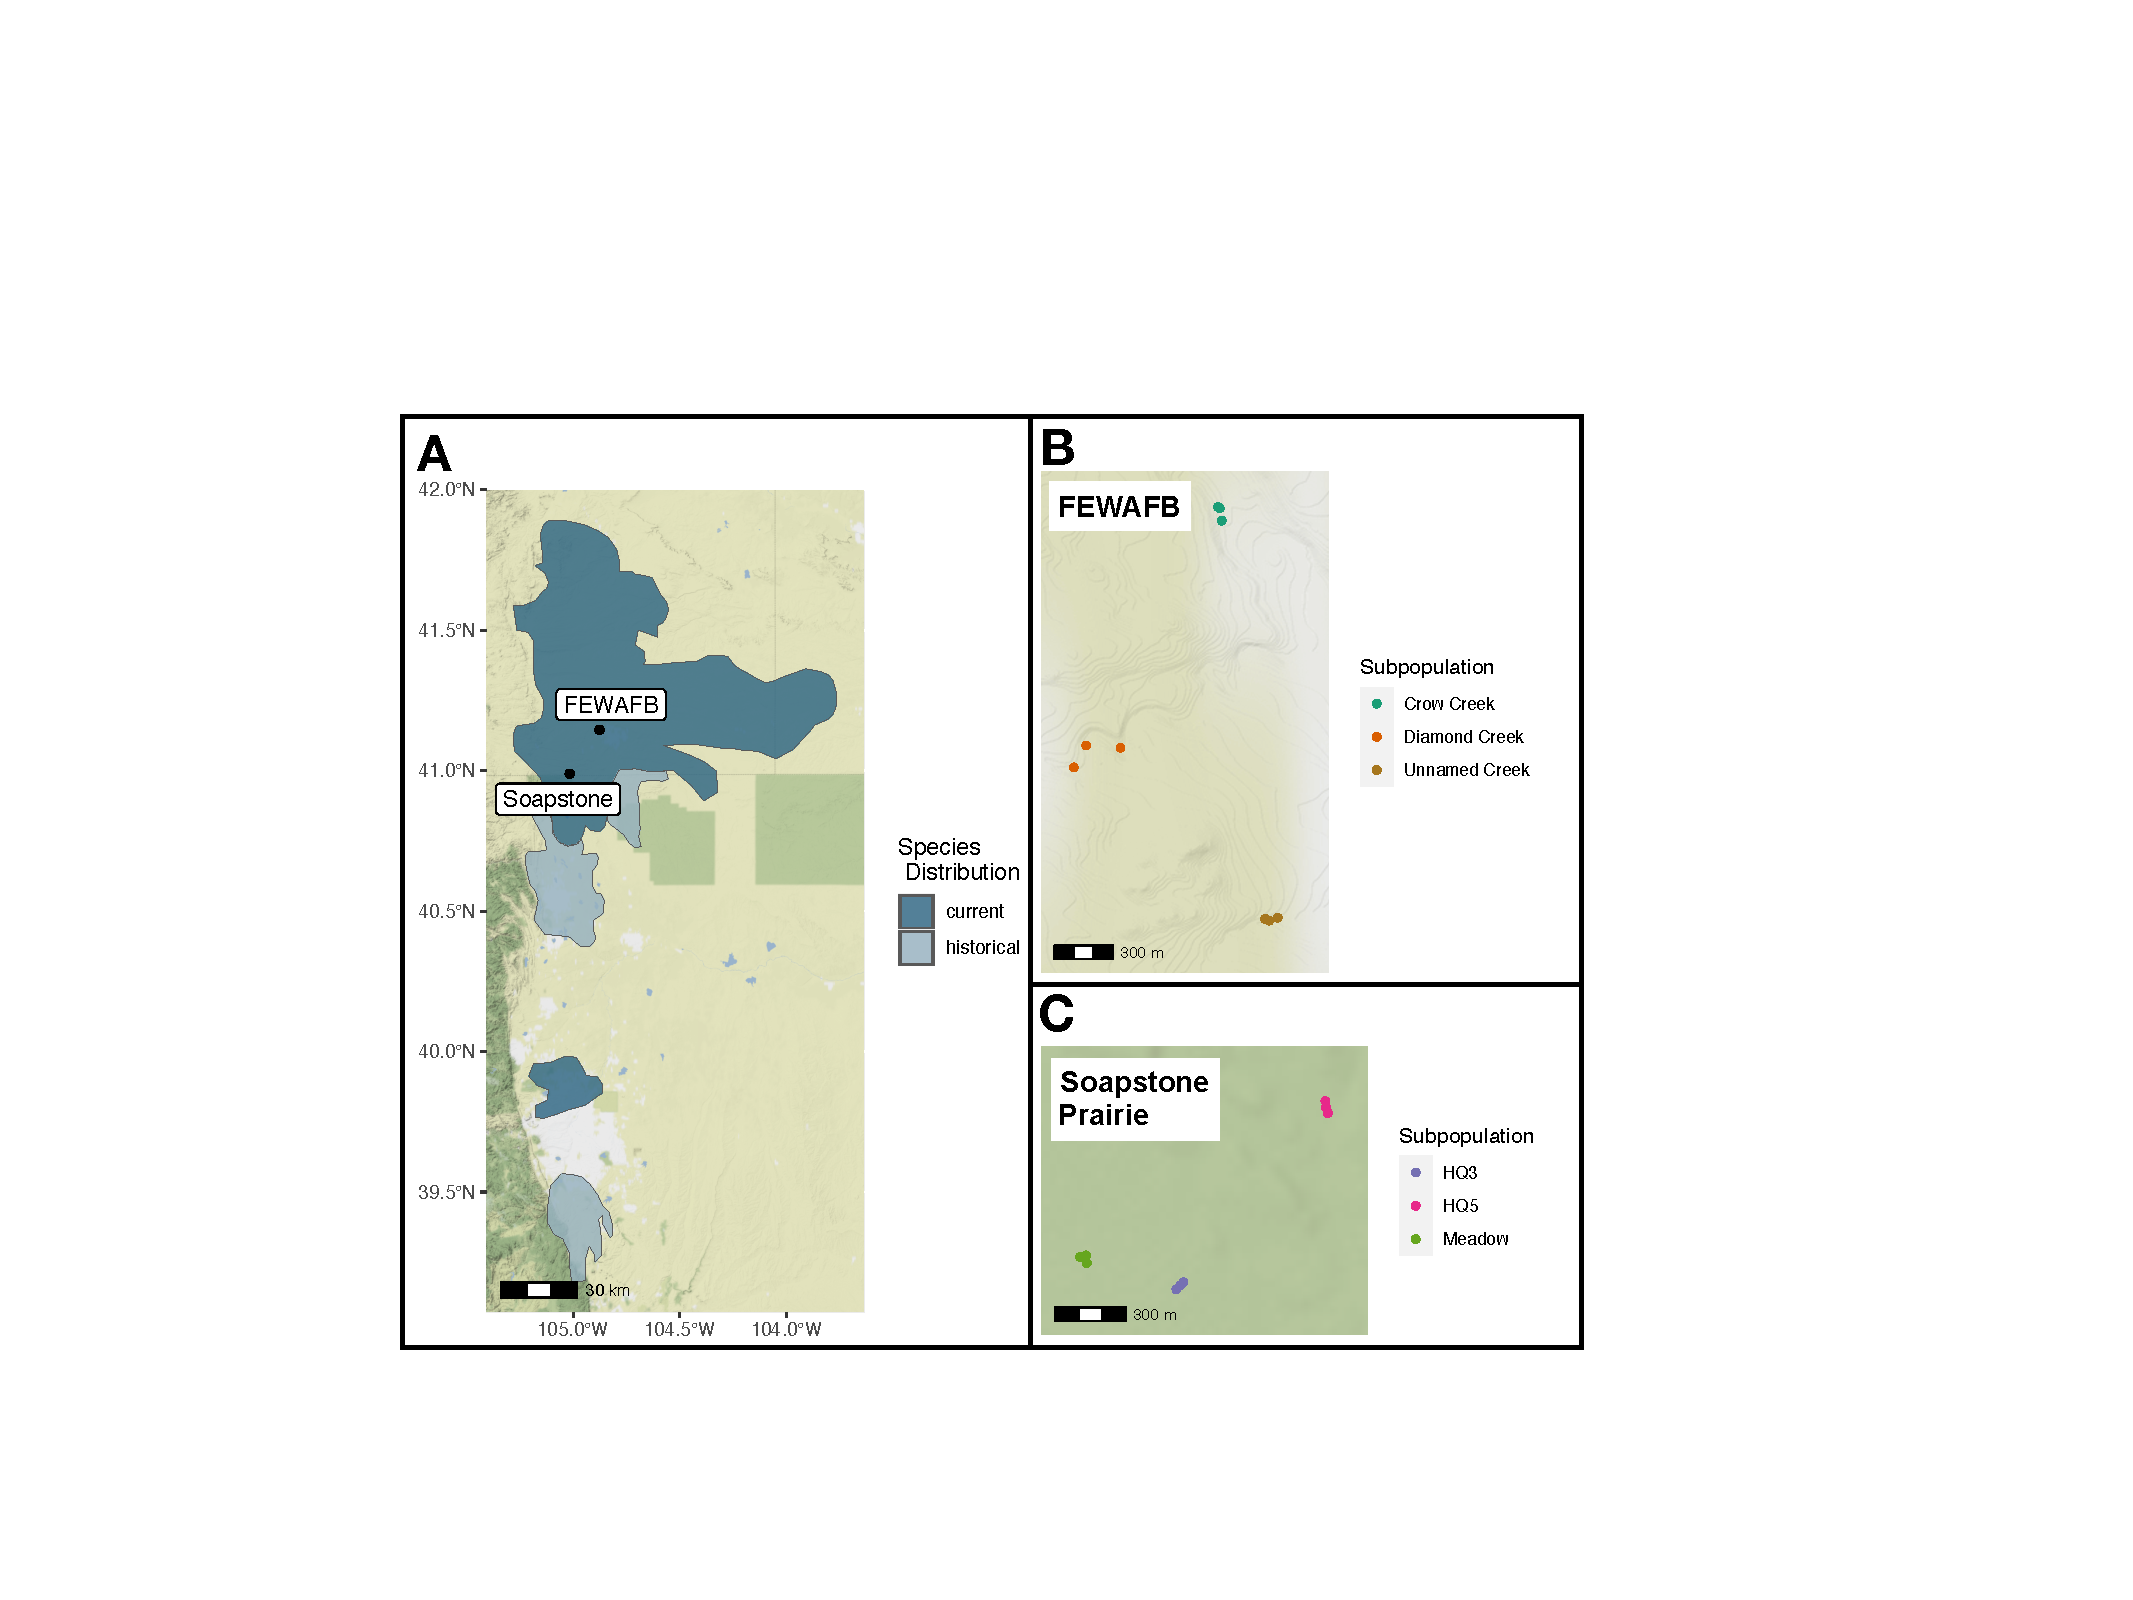
\includegraphics[width = 1\textwidth]{figures/COBP_mapFigure.pdf}
    \caption{\textbf{A} The current known distribution of \textit{O. coloradensis}, shown in dark blue, extends into Wyoming, Colorado, and Nebraska. The historical distribution included the current distribution area as well as some additional locations shown in pale blue. Distribution information comes from Everson, 2019. Black dots show the relative locatino of the FEWAFB and Soapstone prairie populations included in this study. Colored dots show the location of plots in each subpopulation at FEWAFB (\textbf{B}) and Soapstone Prairie (\textbf{C}).}
    \label{fig:plotMap}
\end{figure}

\begin{figure}[h]
  \centering
  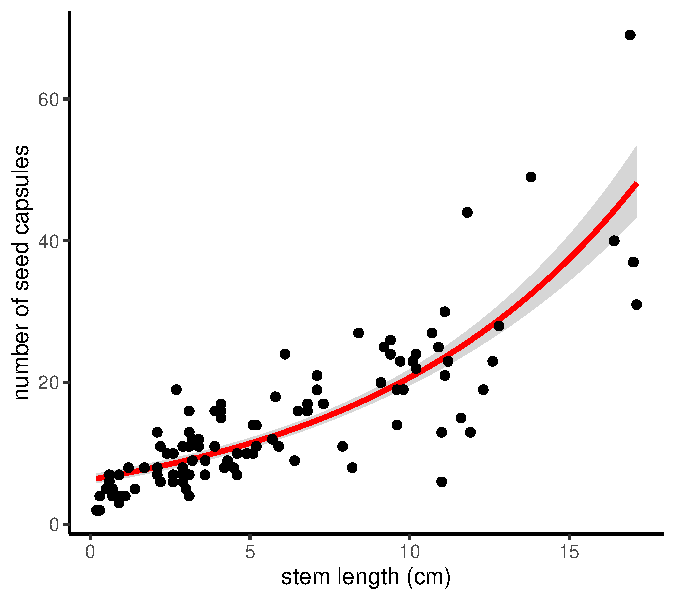
\includegraphics[width=.7\textwidth]{seedRegressionPlot.pdf}
  \caption{As the stem length of an \textit{Oenothera coloradensis} flowering individual increases, the number of capsules it produces increases as well. The red line shows the fit from a Poisson generalized linear model, and the grey ribbon shows the 95\% confidence interval around the fitted relationship. Model equation: Number of capsules = $e^{(1.843 + 0.119\text{\textsf{x}}\text{S}))}$, where \textit{S} is stem length in cm (pseudo R-squared = 0.42, \textit{P} = $<$ 0.01, Resdiual deviance = 186.98, df = 104).  }
  \label{fig:seedRegression}
\end{figure} 

\end{document}